\documentclass[11pt,a4paper]{article}
\usepackage[margin=24mm]{geometry}
\usepackage[T1]{fontenc}
\usepackage{amsmath,amssymb,booktabs,xcolor,enumitem,longtable,tikz,float}
\usepackage[hidelinks]{hyperref}
\setlength{\parindent}{0pt}
\setlength{\parskip}{5pt}
\setlength{\emergencystretch}{2em}
\definecolor{replyblue}{RGB}{20,58,125}
\newcommand{\point}[2]{\par\medskip\textbf{#1}\par\begin{quote}\itshape #2\end{quote}}
\newenvironment{reply}{\begingroup\color{replyblue}\textbf{Reply.} }{\par\endgroup}
\renewcommand{\thetable}{R\arabic{table}}
\renewcommand{\thefigure}{R\arabic{figure}}
% Manually maintained response. Do not rerun the legacy build_response.py over this file.
\begin{document}
\begin{center}
{\Large\bfseries WarpVox: Response to the Editor and Reviewers}\\[5pt]
{Submission 26-4628 --- Revision response}
\end{center}
{\small Tables and figures numbered R1, R2, etc. belong to this response.}

Dear Editor and reviewers,

Thank you for the detailed comments. We have rewritten the Method section and completed the additional evaluations reported below. The response covers:
\begin{itemize}[nosep,leftmargin=*]
\item Explicit definitions, numerical parameters, pseudocode, and a mechanism illustration for the correction pipeline.
\item A matched target-construction comparison with paired results on ten cases, complemented by an ablation of Stage-1 observation association.
\item Repeated correction and continued fusion on nine multi-loop sequences, with 30 post-correction and 21 post-fusion checkpoints.
\item Parameter sensitivity, event-level reconstruction differences, and a precise definition of the video runtimes.
\item ElasticFusion comparisons on TUM RGB-D and Kimera-Multi, and Chamfer distances for the reconstruction and deformation baselines.
\end{itemize}

\section*{Response to the Editor}
The Editor's report is grouped into the four requests below.
\point{Editor E1: clarity and reproducibility}{Substantial revisions are needed to improve methodological clarity and reproducibility. The revision should provide missing algorithmic details and parameters.}
\begin{reply}
Section III specifies the inputs, tests, and update rules of the existing four-stage pipeline. It also explains their design basis: observation support links pose corrections to the fused surface, weighted target construction reconciles the corrected observations, ARAP propagates the constraints while penalizing local distortion, and source-supported reconstruction restores the state needed for continued fusion. The parameter table specifies the fixed and modality-dependent settings, and Algorithm 1 gives the execution order of Stage 3. The revised Method specifies candidate selection, open-boundary handling, and mesh-repair stopping rules. Figure~\ref{fig:reply-mechanisms} illustrates association, component-aware clustering, and output support classes. The sensitivity results in R1-3(c) quantify the effects of the rejection thresholds.
\end{reply}
\par\medskip\textbf{Editor E2: controlled target ablation.}\par
\begin{reply}
We evaluated matched multi-keyframe pose transport on the ten ablation cases, preserving the candidate keyframes, reliability weights, aggregation/trimming, and downstream processing. R1-3(a) reports the paired results and explains the relationship between the two target constructions. Stage 1 reconstructs the observation support of the fused surface; Stage 2 uses this support to turn corrected keyframe poses into surface displacement constraints. The matched comparison tests the candidate-coordinate construction within this shared observation framework. The complementary association ablation in R1-3(c) shows that removing all association gates reduces mean F@25 from 26.75\% to 25.64\%.
\end{reply}
\point{Editor E3: repeated correction and fusion}{Evaluate stability over repeated correction-and-fusion cycles.}
\begin{reply}
The corrected TSDF supports repeated correction and fusion in nine sequences containing two to six loop closures, evaluated at 30 checkpoints immediately after correction and 21 checkpoints after continued fusion. Each reference reintegrates the same measurement history with the corrected poses available at that checkpoint. Mean F@25 differences from reintegration are $+1.38$ and $+1.22$ percentage points at the two checkpoint types. Across the 21 matched fusion intervals, sign agreement increases by 0.79 percentage points and support IoU by 2.79 percentage points on average. R1-3(b) reports the complete checkpoint table and the evolution of surface fidelity and volumetric agreement across successive corrections.
\end{reply}
\point{Editor E4: relation to deformation-based approaches}{Better establish the contribution relative to existing deformation-based approaches.}
\begin{reply}
The submitted manuscript presents WarpVox as a system for correcting an externally maintained TSDF after a trajectory revision and resuming fusion without full reintegration (Sections I--II), and already compares surface correction with Kimera-PGMO (Table III). Kimera-PGMO and ElasticFusion both use embedded deformation graphs, so the existing comparison already covers this deformation-based approach. Under the same input mesh and pre-/post-correction trajectories, WarpVox improves F@25/F@50 by 0.26/0.91 percentage points and reduces surface-correction core time from 8.231 to 3.515\,s. The revision makes the complete map update more explicit: keyframe pose corrections drive an intermediate surface deformation, and reconstruction combines the warped zero set with source-derived support, integration weights, sign, and free space to restore a native TSDF for continued fusion. The additional ElasticFusion comparison and repeated-cycle evaluation further substantiate reconstruction performance and continued fusion, respectively. R2-S2 and R2-S3 provide the details.
\end{reply}
\section*{Response to Reviewer 1}
\point{R1-2: Stage-3 pseudocode}{The four-stage structure is easy to follow, and the introduction clearly motivates the problem. Section III-D is harder to follow because several filtering, target-adjustment, and mesh-repair operations are described in succession. Pseudocode showing their order would help.}
\begin{reply}
Algorithm 1 in Section III-D now gives the execution order of filtering, target consolidation, ARAP deformation, and mesh repair, with references to each step's definition.
\end{reply}
\point{R1-3(a): observation-derived targets}{Table IV reports a 0.637-percentage-point improvement at F@25 over nearest-keyframe pose transport. This is useful evidence, but the comparison does not clearly distinguish the benefit of measured samples from that of combining several keyframes rather than using only the nearest one.

Please add a matched multi-keyframe pose-transport baseline. Keep the candidate keyframes, reliability weights, aggregation/trimming procedure, and downstream processing unchanged. Instead of constructing each candidate target from the matched range sample as in Eq. (3), apply the corresponding keyframe's pre-to-post pose correction to the original source vertex, then aggregate the candidates. Paired results for the individual ablation cases would show how consistently the measured-sample formulation improves on this control.}
\begin{reply}
\textbf{Matched comparison.}
We evaluated the requested control on the ten Kimera-Multi ablation cases at 25\,cm voxel resolution. The candidate keyframes, reliability weights, aggregation/trimming procedure, and downstream processing are identical. Each control candidate applies the associated keyframe's pre-to-post pose correction to the source vertex. The measured-sample formulation achieves mean F@10/F@25/F@50 scores of $10.16/26.63/45.41\%$, compared with $10.04/26.55/45.39\%$ for matched pose transport. Table~\ref{tab:reply-r1a-paired} gives all ten paired differences; F@25 increases in nine cases.

{\small
\begin{longtable}{lrrr}
\caption{Paired target-construction results. $\Delta F$ is the measured-sample score minus the matched pose-transport score, in percentage points.}\label{tab:reply-r1a-paired}\\
\toprule
Case & $\Delta F@10$ & $\Delta F@25$ & $\Delta F@50$\\
\midrule
\endfirsthead
\toprule
Case & $\Delta F@10$ & $\Delta F@25$ & $\Delta F@50$\\
\midrule
\endhead
10\_14 acl\_jackal2, L1 & $+0.20$ & $+0.22$ & $-0.08$\\
10\_14 sparkal1, L1 & $+0.20$ & $+0.12$ & $+0.04$\\
10\_14 sparkal2, L1 & $+0.21$ & $+0.08$ & $+0.06$\\
12\_07 acl\_jackal2, L2 & $-0.33$ & $-0.07$ & $+0.01$\\
12\_07 hathor, L1 & $+0.02$ & $+0.04$ & $-0.10$\\
12\_07 sparkal1, L1 & $+0.18$ & $+0.08$ & $+0.08$\\
12\_08 acl\_jackal2, L1 & $+0.23$ & $+0.13$ & $+0.17$\\
12\_08 apis, L1 & $+0.13$ & $+0.08$ & $-0.01$\\
12\_08 sobek, L1 & $+0.19$ & $+0.04$ & $-0.01$\\
12\_08 thoth, L1 & $+0.17$ & $+0.08$ & $+0.02$\\
\midrule
Mean & $+0.12$ & $+0.08$ & $+0.02$\\
\bottomrule
\end{longtable}
}

\textbf{Reconstructing observation support and displacement constraints.}
TSDF fusion combines posed range observations from multiple frames into a shared distance field through weighted integration (\href{https://arxiv.org/html/1611.03631#S4}{Voxblox, Sec.~IV}). WarpVox follows this construction in reverse at the level of observation support: starting from the fused surface, Stage 1 projects each source vertex into candidate keyframes under the pre-correction poses and retains geometrically consistent measurements. Stage 2 then repositions these measurements under the corrected poses and aggregates them into surface targets. The old poses establish which observations support the existing geometry; the corrected poses determine where those observations move.

The measured-sample construction retains each observation's sensor-frame geometry. For the retained set $I_j$ with nonnegative weights and positive total weight, the target is the unique weighted least-squares solution:
\[
\begin{aligned}
v_j^*&=\operatorname*{argmin}_{x\in\mathbb R^3} E_j(x)
=\frac{\sum_{r\in I_j}\omega_{rj}q_{rj}^{\mathrm{meas}}}{\sum_{r\in I_j}\omega_{rj}},\\
E_j(x)&=\sum_{r\in I_j}\omega_{rj}\|x-q_{rj}^{\mathrm{meas}}\|^2.
\end{aligned}
\]
Indeed, $E_j(x)-E_j(v_j^*)=(\sum_{r\in I_j}\omega_{rj})\|x-v_j^*\|^2$.
In a local plane-distance model with common unit normal $n$, the weighted field of these samples is $D_j(x)=n^\top(x-v_j^*)$, so $D_j(v_j^*)=0$. This connects the target to the fused zero plane of the retained observations in that model. Section III-C now states this construction and its relation to distance fusion.

The matched comparison retains this observation support and tests two ways of constructing candidate target coordinates in Stage 2. Writing the source vertex in the pre-correction keyframe coordinates as $\hat v_{rj}^-$, the two candidates are
\[
\begin{aligned}
q_{rj}^{\mathrm{meas}} &= \widehat R_r^+ m_{rj}+\widehat t_r^+,\\
q_{rj}^{\mathrm{pose}} &= \widehat R_r^+\hat v_{rj}^-+\widehat t_r^+,\\
q_{rj}^{\mathrm{meas}}-q_{rj}^{\mathrm{pose}}
&=\widehat R_r^+(m_{rj}-\hat v_{rj}^-).
\end{aligned}
\]
Here $m_{rj}$ is the associated sensor-frame measurement and $(\widehat R_r^+,\widehat t_r^+)$ is its corrected keyframe pose. Stage 1 bounds $\|m_{rj}-\hat v_{rj}^-\|$ through its association gate. Both constructions apply the same keyframe pose corrections through the reconstructed observation support; their candidate coordinates differ by the rotated association residual. The close F@25 and F@50 scores are consistent with this bounded difference.

\textbf{Direct ablation of observation association.}
The Stage-1 ablation in R1-3(c), Table~\ref{tab:reply-association-gates}, tests the role of observation screening. Removing all association gates reduces mean F@25 from 26.75\% to 25.64\%. This experiment directly evaluates the geometric verification that establishes the observation support shared by both Stage-2 constructions.

\textbf{Contribution.}
WarpVox reconstructs the observation support of an already fused surface and uses it to convert back-end pose corrections into deformation constraints. Source-supported reconstruction combines the corrected surface with the volume's observed support, integration weights, sign information, and free space to produce a native TSDF for continued fusion. The original Nearest-KF comparison evaluates the observation-guided target construction against assigning each control the correction of its spatially nearest keyframe.
\end{reply}
\point{R1-3(b): repeated correction and fusion}{Section IV-A already describes sequential processing with fusion resumed from the corrected volume, and Section IV-D reports volumetric consistency. However, the averages do not show how discrepancies evolve over successive correction-and-fusion cycles within a sequence. For a few existing sequences with multiple loop closures, please report the difference in GT-referenced surface scores relative to full reintegration, together with the existing volumetric-consistency metrics, over successive events. Checkpoints immediately after correction and after a specified interval of additional fusion would help distinguish the two stages. The reference should use the same measurement history and corrected poses. Since distance values are reconstructed and source-derived support and weights are transferred repeatedly, this analysis would help establish whether the approximation remains stable during continued use. Exact equivalence with reintegration is not required.}
\begin{reply}
The submitted Section IV-A already describes fusion resumed from the corrected TSDF. The additional experiment quantifies its evolution over successive correction-and-fusion cycles on nine Kimera-Multi sequences containing 30 loop closures. Checkpoint A is taken immediately after each correction. Checkpoint B is taken after integrating the subsequent frames up to the next loop closure, before applying that next correction. The fusion interval is therefore event-defined and varies between loop pairs. Processing ends at the final correction, yielding 30 A and 21 B checkpoints. At each checkpoint, the reference uses the same frames and the same corrected poses as WarpVox.

Let $\Delta F=F_{\mathrm{WarpVox}}-F_{\mathrm{reint}}$, measured in percentage points. The aggregate results are:
\begin{center}\small
\begin{tabular}{lrrrrr}\toprule
Checkpoint & $n$ & Mean $\Delta F@25$ & Range & Sign (\%) & Support IoU (\%)\\\midrule
A: after correction & 30 & $+1.38$ & $[-1.10,+4.56]$ & 91.7 & 78.8\\
B: after fusion & 21 & $+1.22$ & $[-1.24,+4.58]$ & 93.8 & 83.5\\\bottomrule
\end{tabular}
\end{center}
Table~\ref{tab:reply-cycles} reports both F@25 scores and their paired difference at every checkpoint in sequence order. Support IoU compares positive-weight voxel sets; sign agreement measures consistency of the signed-distance fields under the evaluation mask. The A and B averages summarize different checkpoint sets. Comparing each B with its preceding A instead gives mean improvements of 0.79 percentage points in sign agreement and 2.79 percentage points in support IoU over the 21 fusion intervals.

The other surface metrics follow the same evaluation protocol. Mean WarpVox-minus-reintegration differences at A are $+0.86$ and $+1.18$ percentage points for F@10 and F@50, and $-0.1$\,cm for Chamfer distance. At B, they are $+0.71$, $+1.02$ percentage points, and $+0.6$\,cm, respectively. Lower Chamfer distance is better. These are checkpoint-wise paired differences, averaged over the indicated checkpoint set.

The six-loop 12\_07 hathor sequence illustrates the distinction between surface fidelity and volumetric agreement. Its $\Delta F@25$ is $+2.50$ percentage points after the first correction and $+3.17$ after the sixth. Over these checkpoints, support IoU changes from 83.6\% to 67.3\%, and sign agreement from 92.2\% to 82.9\%. WarpVox maintains higher F@25 than reintegration at all six post-correction checkpoints; the support and sign measurements describe the accompanying volumetric agreement.

The reconstruction recomputes distances from the warped surface and transfers available source weights, capped at $w_{\max}=10^4$. Voxels supported by the geometric fallback receive a geometric prior weight for continued fusion. Subsequent observations update these distance--weight pairs by standard weighted TSDF integration. This retains the source volume's accumulated evidence while incorporating new measurements into the corrected geometry.
\end{reply}
\point{R1-3(c): reproducibility and sensitivity}{Eqs. (4)-(6) specify the aggregation and trimming rules, but I could not find the explicit function mapping the correspondence cues to alpha\_\{rj\} in Section III-B, or the numerical values of epsilon\_m and kappa in Eq. (5). Some neighbourhood definitions and thresholds for median-MAD rejection, Welsch-based target consolidation, and mesh repair in Section III-D also remain unspecified. Please provide these settings in a compact table and indicate which are fixed across datasets and voxel resolutions. The text already states that kappa is shared across modalities; the remaining settings need similar clarification. A small sensitivity test for one or two influential rejection thresholds would help assess how much the results depend on tuning.}
\begin{reply}
The association reliability is defined in Section III-B and reproduced in R2-B3. Section III-C specifies the aggregation weights and trimming rule. The fixed settings include the following:
\begin{center}\small
\begin{tabular}{p{0.37\linewidth}p{0.55\linewidth}}\toprule
Quantity & Setting\\\midrule
Association range & $0.1$--$10$\,m (RGB-D); $0.5$--$80$\,m (LiDAR)\\
Measurement gate $g_0+g_1z^-$ & $0.08+0.01z^-$\,m (RGB-D); $0.25+0.003z^-$\,m (LiDAR)\\
Reliability scales $(\sigma_g,\sigma_z,z_0)$ & $(0.048,0.08,8)$\,m (RGB-D); $(0.15,\text{--},40)$\,m (LiDAR)\\
Target damping scale $\zeta_m$ & $3$\,m (RGB-D); $20$\,m (LiDAR)\\
Stage-2 trimming & $\kappa=2.5$; $\epsilon_m=0.02$\,m (RGB-D), $0.05$\,m (LiDAR)\\
Control prediction and rejection & $k=20$, $n_{\min}=16$, $\gamma=1.5$, $\sigma_{\min}=0.05$\,m\\
Fragments and proxy & $N_{\rm f}=100$ faces; $P_{\max}=60{,}000$; proxy above $1.3P_{\max}$ source vertices\\
Welsch consolidation & 4 rounds; $c_{\rm g}=4.685$; at least 6 fitting neighbours\\
ARAP & 20 local--global iterations\\
Mesh repair & Edge/area/aspect bounds $3/6/20$; long-edge threshold $0.5$\,m; at most 3 passes and 80 Jacobi steps per pass\\
TSDF reconstruction & $\tau=4s$, $\rho=1.5s$, $\tau_{\rm fs}=1.5s$, face search radius $16s$, $w_{\max}=10^4$\\\bottomrule
\end{tabular}
\end{center}
These settings are fixed across datasets and voxel resolutions, with modality-specific values identified in the parameter table. Distances expressed as multiples of voxel size $s$ scale with the grid resolution.

For observation $r$ of vertex $j$, the aggregation weight is
\[
\omega_{rj}=\begin{cases}
\alpha_{rj}/(1+z^m_{rj}/\zeta_m), & \text{RGB-D},\\
\alpha_{rj}/(1+\|q_{rj}^+-v_j^-\|/\zeta_m), & \text{LiDAR},
\end{cases}
\]
where $q_{rj}^+$ is the matched sensor sample transformed by the corrected keyframe pose. The initial target $\bar q_j$ is its weighted mean over observations with valid corrected poses. We retain samples whose residual from $\bar q_j$ is at most $\max(\epsilon_m,\kappa\,\operatorname{median}_r\|q_{rj}^+-\bar q_j\|)$ and recompute the weighted mean. With fewer than three valid samples, all are retained. R2-D3--D4 and R2-D11 specify the neighbourhood and robust rejection rules; R2-D18 gives the repair tests.

We tested the RGB-D association gate and reliability cutoff on ten ablation cases, changing one setting at a time. The default mean F@25 for this sweep is 26.735\%. The paired changes are:
\begin{center}\small
\begin{tabular}{lrrr}\toprule
Change & Mean $\Delta F@25$ (pp) & Case range (pp) & $\Delta$CD (cm)\\\midrule
$g_0:0.08\to0.04$\,m & $-0.037$ & $[-0.18,+0.07]$ & $-0.12$\\
$g_0:0.08\to0.16$\,m & $-0.065$ & $[-0.29,+0.10]$ & $+0.01$\\
$\alpha_{\min}:0.05\to0$ & $-0.030$ & $[-0.54,+0.33]$ & $-0.36$\\
$\alpha_{\min}:0.05\to0.20$ & $-0.190$ & $[-0.52,0.00]$ & $+0.06$\\\bottomrule
\end{tabular}
\end{center}
The same experiment varies the Stage-3 MAD multiplier, scale floor, neighbourhood, Welsch cutoff, and repair settings. Across the tested Stage-3 settings, mean F@25 changes by $-0.021$ to $+0.046$ percentage points; the stricter association-reliability cutoff has the larger effect on these cases.

\textbf{Role of Stage-1 observation screening.}
A complementary ablation removes all Stage-1 association gates while retaining the downstream pipeline. Table~\ref{tab:reply-association-gates} compares this variant with its default on the same ten cases. Geometric verification raises mean F@25 by 1.11 percentage points, from 25.64\% to 26.75\%. On 12\_07 acl\_jackal2, L2, the corresponding scores are 52.77\% and 65.89\%, a 13.12-percentage-point improvement. These results demonstrate the role of observation screening in establishing the surface-to-keyframe constraints used for correction.

{\small
\begin{longtable}{lrrrr}
\caption{Stage-1 association ablation on ten cases. CD is in centimetres.}\label{tab:reply-association-gates}\\
\toprule
Association setting & F@10 (\%) & F@25 (\%) & F@50 (\%) & CD\\
\midrule
Geometrically verified (default) & 10.16 & 26.75 & 45.54 & 101.7\\
All association gates removed & 8.93 & 25.64 & 45.40 & 103.8\\
\bottomrule
\end{longtable}
}

A separate Stage-2 sweep holds its upstream observations fixed and varies $\kappa\in\{1.5,4.0\}$ and $\epsilon_m\in\{0.01,0.05\}$\,m around the RGB-D default. Its default mean F@25 is 26.63\%; the largest absolute case-level change is 0.07 percentage points. At the default, trimming rejects candidates at 23.0\% of eligible vertices, removing 5.32\% of their candidates. Changing $\kappa$ from 1.5 to 4.0 changes the affected-vertex fraction from 58.1\% to 6.8\%. Under the default, the per-case median target changes at affected vertices are 3.8--6.2\,mm. These millimetre-scale adjustments explain the stable F@25 scores at 25\,cm voxel resolution. Each sweep is compared with its own default run.
\end{reply}
\point{R1-4: dataset means and event-level differences}{The abstract's statement about remaining within 0.32 percentage points of reintegration at F@25 appears to refer to the dataset means in Table I. Please make this explicit unless the same bound is established for individual loop events. Case-level differences would make occasional deteriorations visible alongside the mean improvements.}
\begin{reply}
The 0.32-percentage-point value refers to the dataset means. We replace the abstract sentence with:
\begin{quote}
Across 39 Kimera-Multi and 12 KITTI loop-closure cases, the dataset-mean F@25 scores differ from full reintegration by $+0.05$ and $-0.32$ percentage points, respectively, while RGB-D mean core update time decreases from 109.25 to 2.26\,s.
\end{quote}
The event-level differences make the variation around these means explicit:
\begin{center}\small
\begin{tabular}{lrrrrr}\toprule
Setting & Cases & Mean $\Delta$ (pp) & Minimum & Maximum & Cases with $\Delta<0$\\\midrule
Kimera, 25\,cm & 39 & $+0.05$ & $-2.91$ & $+2.59$ & 22\\
KITTI, 25\,cm & 12 & $-0.32$ & $-3.03$ & $+1.80$ & 8\\
Kimera, 10\,cm & 11 & $+0.09$ & $-4.53$ & $+2.35$ & 4\\\bottomrule
\end{tabular}
\end{center}
Here $\Delta$ is the WarpVox-minus-reintegration F@25 difference for the same event. Table~\ref{tab:reply-event-deltas} lists all events underlying these summaries, distinguishing the dataset means from the range of individual corrections.
\end{reply}
\point{R1-6: video runtime}{The video helps illustrate map correction and continued fusion. Please clarify which processing steps are included in the displayed runtimes and how they relate to the in-memory core-update times reported in the paper.}
\begin{reply}
The WarpVox annotation indicates approximate core map-update time for Stages 1--4, using the same timing scope as the paper and excluding I/O and visualization. The ``bag t'' label in the Voxblox footage indicates elapsed time in the recorded sequence, not computation time.
\end{reply}
\section*{Response to Reviewer 2}


\point{R2-S1: Methodological clarity and reproducibility}{There are many inconsistent and vague descriptions that make it impossible for a reader to reproduce the method based on the manuscript alone.}
\begin{reply}
The revised Section III makes the definitions and update rules explicit. Table I collects the parameters, and Algorithm 1 gives the Stage-3 execution order; the replies below address the specific questions.
\end{reply}
\point{R2-S2: Conceptual distinction from ElasticFusion}{The difference seems to be the use of triangles in place of surfels for computing the deformations.}
\begin{reply}
WarpVox is a map-correction system that updates an externally maintained TSDF after a back-end trajectory revision and returns a native TSDF ready for continued fusion, without full reintegration. This input--output distinction is already described in Sections I--II of the submitted manuscript. Within this system, Stage 1 associates the fused surface with keyframe observations; Stage 2 repositions and aggregates the associated measurements under the corrected poses to construct deformation targets. The triangle mesh carries this surface deformation between the input and output TSDFs. Its reconstruction combines distances from the warped surface with source-derived support, sign, integration weights, and free space, preserving the volumetric state needed to resume TSDF fusion. ElasticFusion and Kimera-PGMO both use embedded deformation graphs: ElasticFusion derives constraints from local and global surface registration within its surfel SLAM system, while Kimera-PGMO propagates trajectory corrections to a timestamped mesh. ARAP and QEM provide WarpVox's deformation machinery. The submitted Table III already compares surface correction with this deformation-graph approach through Kimera-PGMO under the same input mesh and pre-/post-correction trajectories: WarpVox improves F@25/F@50 by 0.26/0.91 percentage points with a $2.34\times$ speedup in surface correction. Stage 4 then reconstructs a native TSDF in another 1.277\,s, for 4.792\,s in total. The repeated-cycle experiment further demonstrates that the resulting volume supports subsequent fusion and correction.
\end{reply}
\point{R2-S3: ElasticFusion evaluation}{I suggest clarifying the conceptual difference to ElasticFusion, and comparing performance against ElasticFusion, rather than VoxBlox reintegration or VoxGraph.}
\begin{reply}
The submitted Table III already evaluates embedded-deformation-based correction through Kimera-PGMO under the same initial mesh and pre-/post-correction trajectories. This comparison covers the deformation-graph approach also used by ElasticFusion. Sections I--II already describe WarpVox's correction of an externally maintained TSDF and return to continued fusion without full reintegration; R2-S2 above details this system design. The additional ElasticFusion results below reinforce this existing comparison on TUM fr3/long\_office\_household and ten Kimera-Multi sequences. ElasticFusion uses its own tracking; WarpVox and Voxblox reintegration use ORB-SLAM3 poses.

On TUM, WarpVox achieves F@2 of 72.13\% and Chamfer distance of 2.82\,cm, compared with 62.77\% and 3.69\,cm for ElasticFusion. ElasticFusion's absolute trajectory error (ATE) RMSE is 1.80\,cm; the ORB-SLAM3 trajectory used by the TSDF methods achieves 1.01\,cm. The map reference is reconstructed from RGB-D measurements with motion-capture poses. The reconstruction scores are:
\begin{center}\small
\begin{tabular}{lrrrr}\toprule
Method & F@1 (\%) & F@2 (\%) & F@5 (\%) & CD (cm)\\\midrule
ElasticFusion & 33.17 & 62.77 & 83.44 & 3.69\\
Voxblox reintegration & 33.23 & 68.64 & 89.04 & 2.99\\
WarpVox & 37.61 & 72.13 & 89.53 & 2.82\\\bottomrule
\end{tabular}
\end{center}
The F-score thresholds are in centimetres.

On Kimera-Multi, maps are compared at the last evaluated loop event in each sequence:
\begin{center}\small
\begin{tabular}{lrrrr}\toprule
Method & F@10 (\%) & F@25 (\%) & F@50 (\%) & CD (m)\\\midrule
ElasticFusion & 0.69 & 1.98 & 3.86 & 37.72\\
Voxblox reintegration & 8.18 & 24.29 & 44.13 & 1.03\\
WarpVox & 8.16 & 23.68 & 43.18 & 1.04\\\bottomrule
\end{tabular}
\end{center}
ElasticFusion's mean trajectory ATE is 115.785\,m in these runs.

\end{reply}
\subsection*{General}

\point{R2-G1}{Please expand the acronym on first use.}
\begin{reply}
The revision expands abbreviations on first use in both the abstract and the main text.
\end{reply}

\point{R2-G2}{Illustrate the clustering, association, and different classes of "support" graphically.}
\begin{reply}
Figure~\ref{fig:reply-mechanisms} illustrates observation association, component-aware clustering, and how paired surface frames combine corrected geometry with source TSDF state for continued fusion. Panel (c) also distinguishes the output support classes.
\end{reply}

\begin{figure}[H]
\centering
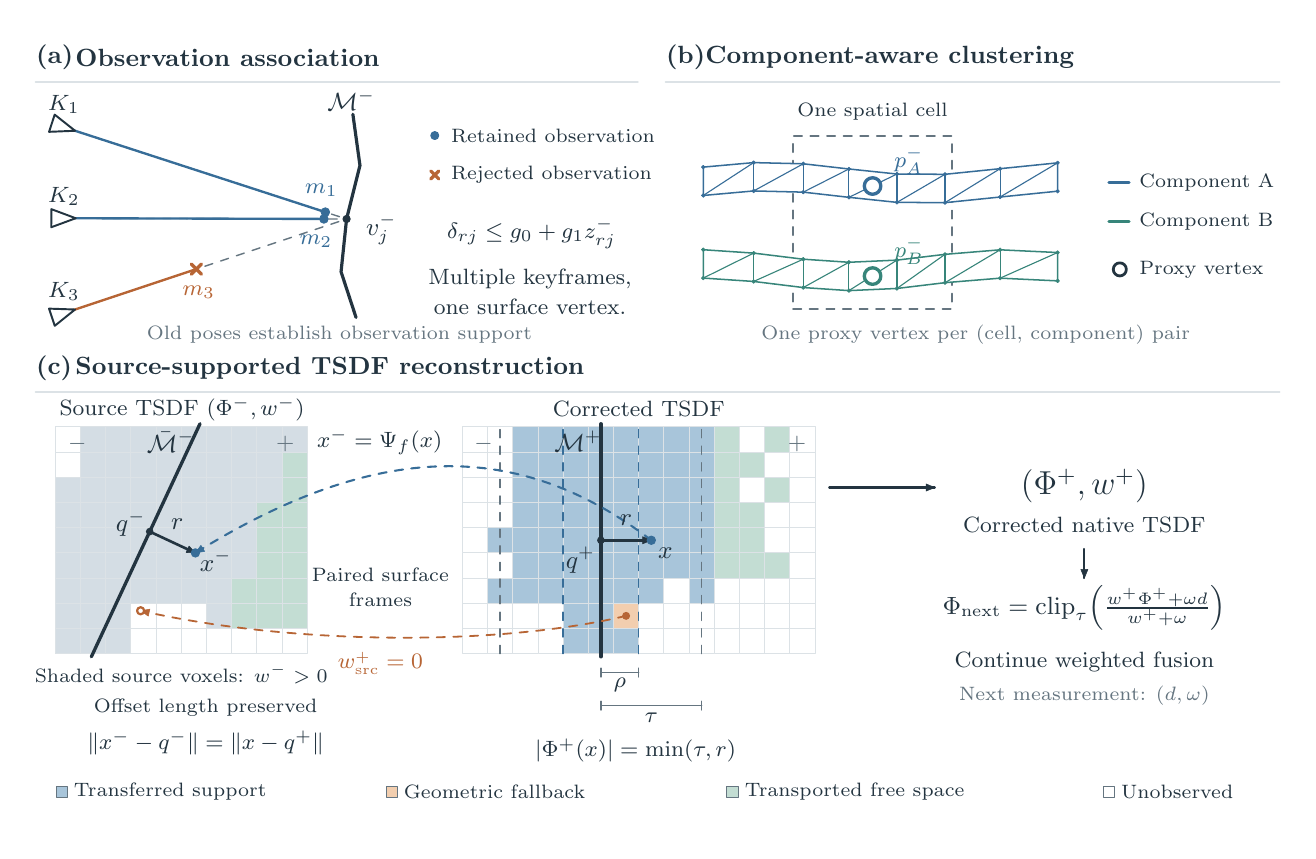
\begin{tikzpicture}[x=1cm,y=1cm,line cap=round,line join=round]
\path[use as bounding box] (0,0) rectangle (16.0,10.2);
\definecolor{wvink}{HTML}{233440}
\definecolor{wvmuted}{HTML}{657580}
\definecolor{wvgrid}{HTML}{DCE2E6}
\definecolor{wvblue}{HTML}{376D98}
\definecolor{wvbluefill}{HTML}{A8C5DA}
\definecolor{wvpale}{HTML}{E8F0F6}
\definecolor{wvteal}{HTML}{37857A}
\definecolor{wvtealfill}{HTML}{C3DDD3}
\definecolor{wvorange}{HTML}{B76535}
\definecolor{wvorangefill}{HTML}{F2CEAF}
\definecolor{wvwhite}{HTML}{FFFFFF}
\definecolor{wvgate}{HTML}{F2F5F7}
\definecolor{wvsource}{HTML}{D4DDE4}
\node[anchor=west,inner sep=0pt,text=wvink,font={\fontsize{9}{10}\selectfont\bfseries}] at (0.1000,9.8200) {(a)};
\node[anchor=west,inner sep=0pt,text=wvink,font={\fontsize{8.6}{9.6}\selectfont\bfseries}] at (0.6000,9.8200) {Observation association};
\draw[draw=wvgrid,line width=0.6pt] (0.1000,9.5100) -- (7.7500,9.5100);
\node[anchor=west,inner sep=0pt,text=wvink,font={\fontsize{9}{10}\selectfont\bfseries}] at (8.1000,9.8200) {(b)};
\node[anchor=west,inner sep=0pt,text=wvink,font={\fontsize{8.6}{9.6}\selectfont\bfseries}] at (8.6000,9.8200) {Component-aware clustering};
\draw[draw=wvgrid,line width=0.6pt] (8.1000,9.5100) -- (15.9000,9.5100);
\node[anchor=west,inner sep=0pt,text=wvink,font={\fontsize{9}{10}\selectfont\bfseries}] at (0.1000,5.8800) {(c)};
\node[anchor=west,inner sep=0pt,text=wvink,font={\fontsize{8.6}{9.6}\selectfont\bfseries}] at (0.6000,5.8800) {Source-supported TSDF reconstruction};
\draw[draw=wvgrid,line width=0.6pt] (0.1000,5.5700) -- (15.9000,5.5700);
\draw[draw=wvink,line width=1.15pt] (4.1700,6.5200) -- (3.9800,7.1000) -- (4.0500,7.7700) -- (4.2200,8.4500) -- (4.1300,9.1000);
\draw[draw=wvmuted,line width=0.5pt,dashed] (0.4500,8.9400) -- (4.0500,7.7700);
\draw[draw=wvblue,line width=0.85pt] (0.4500,8.9400) -- (3.7800,7.8577);
\draw[fill=wvwhite,draw=wvink,line width=0.7pt] (0.2718,8.8770) -- (0.6022,8.8905) -- (0.3429,9.0957) -- cycle;
\node[anchor=center,inner sep=0pt,text=wvink,font={\fontsize{8.3}{9.3}\selectfont}] at (0.4600,9.2200) {$K_1$};
\draw[fill=wvblue,draw=wvblue,line width=0.3pt] (3.7800,7.8577) circle (0.0550);
\draw[draw=wvmuted,line width=0.5pt,dashed] (0.4500,7.7800) -- (4.0500,7.7700);
\draw[draw=wvblue,line width=0.85pt] (0.4500,7.7800) -- (3.7620,7.7708);
\draw[fill=wvwhite,draw=wvink,line width=0.7pt] (0.2997,7.6654) -- (0.6100,7.7796) -- (0.3003,7.8954) -- cycle;
\node[anchor=center,inner sep=0pt,text=wvink,font={\fontsize{8.3}{9.3}\selectfont}] at (0.4600,8.0600) {$K_2$};
\draw[fill=wvblue,draw=wvblue,line width=0.3pt] (3.7620,7.7708) circle (0.0550);
\draw[draw=wvmuted,line width=0.5pt,dashed] (0.4500,6.5700) -- (4.0500,7.7700);
\draw[draw=wvorange,line width=0.85pt] (0.4500,6.5700) -- (2.1420,7.1340);
\draw[fill=wvwhite,draw=wvink,line width=0.7pt] (0.3441,6.4135) -- (0.6018,6.6206) -- (0.2713,6.6317) -- cycle;
\node[anchor=center,inner sep=0pt,text=wvink,font={\fontsize{8.3}{9.3}\selectfont}] at (0.4600,6.8500) {$K_3$};
\draw[draw=wvorange,line width=1.2pt] (2.0770,7.0690) -- (2.2070,7.1990);
\draw[draw=wvorange,line width=1.2pt] (2.0770,7.1990) -- (2.2070,7.0690);
\draw[fill=wvink,draw=wvink,line width=0.4pt] (4.0500,7.7700) circle (0.0450);
\node[anchor=west,inner sep=0pt,text=wvink,font={\fontsize{8.7}{9.7}\selectfont}] at (4.2900,7.6400) {$v_j^-$};
\node[anchor=center,inner sep=0pt,text=wvink,font={\fontsize{9}{10}\selectfont}] at (4.1100,9.2800) {$\mathcal{M}^-$};
\node[anchor=center,inner sep=0pt,text=wvblue,font={\fontsize{8}{9}\selectfont}] at (3.7300,8.1377) {$m_1$};
\node[anchor=center,inner sep=0pt,text=wvblue,font={\fontsize{8}{9}\selectfont}] at (3.6620,7.4908) {$m_2$};
\node[anchor=center,inner sep=0pt,text=wvorange,font={\fontsize{8}{9}\selectfont}] at (2.1720,6.8440) {$m_3$};
\draw[fill=wvblue,draw=wvblue,line width=0.4pt] (5.1700,8.8300) circle (0.0500);
\node[anchor=west,inner sep=0pt,text=wvink,font={\fontsize{7.5}{8.5}\selectfont}] at (5.3700,8.8300) {Retained observation};
\draw[draw=wvorange,line width=1.2pt] (5.1200,8.2800) -- (5.2200,8.3800);
\draw[draw=wvorange,line width=1.2pt] (5.1200,8.3800) -- (5.2200,8.2800);
\node[anchor=west,inner sep=0pt,text=wvink,font={\fontsize{7.5}{8.5}\selectfont}] at (5.3700,8.3300) {Rejected observation};
\node[anchor=center,inner sep=0pt,text=wvink,font={\fontsize{8}{9}\selectfont}] at (6.4000,7.5900) {$\delta_{rj}\leq g_0+g_1z_{rj}^-$};
\node[anchor=center,inner sep=0pt,text=wvink,font={\fontsize{7.7}{8.7}\selectfont}] at (6.3800,7.0100) {Multiple keyframes,};
\node[anchor=center,inner sep=0pt,text=wvink,font={\fontsize{7.7}{8.7}\selectfont}] at (6.3800,6.6600) {one surface vertex.};
\node[anchor=center,inner sep=0pt,text=wvmuted,font={\fontsize{7.5}{8.5}\selectfont}] at (3.9600,6.3000) {Old poses establish observation support};
\draw[draw=wvmuted,line width=0.65pt,dashed] (9.7200,6.6300) -- (11.7400,6.6300) -- (11.7400,8.8200) -- (9.7200,8.8200) -- (9.7200,6.6300);
\node[anchor=center,inner sep=0pt,text=wvink,font={\fontsize{7.4}{8.4}\selectfont}] at (10.7300,9.1300) {One spatial cell};
\draw[fill=wvwhite,draw=wvblue,line width=0.55pt] (8.5800,8.4290) -- (9.2200,8.4863) -- (9.8500,8.4711) -- (10.4300,8.4053) -- (11.0400,8.3412) -- (11.6500,8.3376) -- (12.3500,8.4091) -- (13.0800,8.4832) -- (13.0800,8.1232) -- (12.3500,8.0491) -- (11.6500,7.9776) -- (11.0400,7.9812) -- (10.4300,8.0453) -- (9.8500,8.1111) -- (9.2200,8.1263) -- (8.5800,8.0690) -- cycle;
\draw[draw=wvblue,line width=0.4pt] (8.5800,8.4290) -- (8.5800,8.0690);
\draw[draw=wvblue,line width=0.4pt] (8.5800,8.0690) -- (9.2200,8.4863);
\draw[fill=wvblue,draw=wvblue,line width=0.2pt] (8.5800,8.4290) circle (0.0240);
\draw[fill=wvblue,draw=wvblue,line width=0.2pt] (8.5800,8.0690) circle (0.0240);
\draw[draw=wvblue,line width=0.4pt] (9.2200,8.4863) -- (9.2200,8.1263);
\draw[draw=wvblue,line width=0.4pt] (9.2200,8.1263) -- (9.8500,8.4711);
\draw[fill=wvblue,draw=wvblue,line width=0.2pt] (9.2200,8.4863) circle (0.0240);
\draw[fill=wvblue,draw=wvblue,line width=0.2pt] (9.2200,8.1263) circle (0.0240);
\draw[draw=wvblue,line width=0.4pt] (9.8500,8.4711) -- (9.8500,8.1111);
\draw[draw=wvblue,line width=0.4pt] (9.8500,8.1111) -- (10.4300,8.4053);
\draw[fill=wvblue,draw=wvblue,line width=0.2pt] (9.8500,8.4711) circle (0.0240);
\draw[fill=wvblue,draw=wvblue,line width=0.2pt] (9.8500,8.1111) circle (0.0240);
\draw[draw=wvblue,line width=0.4pt] (10.4300,8.4053) -- (10.4300,8.0453);
\draw[draw=wvblue,line width=0.4pt] (10.4300,8.0453) -- (11.0400,8.3412);
\draw[fill=wvblue,draw=wvblue,line width=0.2pt] (10.4300,8.4053) circle (0.0240);
\draw[fill=wvblue,draw=wvblue,line width=0.2pt] (10.4300,8.0453) circle (0.0240);
\draw[draw=wvblue,line width=0.4pt] (11.0400,8.3412) -- (11.0400,7.9812);
\draw[draw=wvblue,line width=0.4pt] (11.0400,7.9812) -- (11.6500,8.3376);
\draw[fill=wvblue,draw=wvblue,line width=0.2pt] (11.0400,8.3412) circle (0.0240);
\draw[fill=wvblue,draw=wvblue,line width=0.2pt] (11.0400,7.9812) circle (0.0240);
\draw[draw=wvblue,line width=0.4pt] (11.6500,8.3376) -- (11.6500,7.9776);
\draw[draw=wvblue,line width=0.4pt] (11.6500,7.9776) -- (12.3500,8.4091);
\draw[fill=wvblue,draw=wvblue,line width=0.2pt] (11.6500,8.3376) circle (0.0240);
\draw[fill=wvblue,draw=wvblue,line width=0.2pt] (11.6500,7.9776) circle (0.0240);
\draw[draw=wvblue,line width=0.4pt] (12.3500,8.4091) -- (12.3500,8.0491);
\draw[draw=wvblue,line width=0.4pt] (12.3500,8.0491) -- (13.0800,8.4832);
\draw[fill=wvblue,draw=wvblue,line width=0.2pt] (12.3500,8.4091) circle (0.0240);
\draw[fill=wvblue,draw=wvblue,line width=0.2pt] (12.3500,8.0491) circle (0.0240);
\draw[draw=wvblue,line width=0.4pt] (13.0800,8.4832) -- (13.0800,8.1232);
\draw[fill=wvblue,draw=wvblue,line width=0.2pt] (13.0800,8.4832) circle (0.0240);
\draw[fill=wvblue,draw=wvblue,line width=0.2pt] (13.0800,8.1232) circle (0.0240);
\draw[fill=wvwhite,draw=wvblue,line width=1.2pt] (10.7300,8.1890) circle (0.1050);
\node[anchor=west,inner sep=0pt,text=wvblue,font={\fontsize{8.5}{9.5}\selectfont}] at (11.0000,8.5090) {$p_A^-$};
\draw[fill=wvwhite,draw=wvteal,line width=0.55pt] (8.5800,7.3798) -- (9.2200,7.3368) -- (9.8500,7.2595) -- (10.4300,7.2205) -- (11.0400,7.2480) -- (11.6500,7.3212) -- (12.3500,7.3787) -- (13.0800,7.3442) -- (13.0800,6.9842) -- (12.3500,7.0187) -- (11.6500,6.9612) -- (11.0400,6.8880) -- (10.4300,6.8605) -- (9.8500,6.8995) -- (9.2200,6.9768) -- (8.5800,7.0198) -- cycle;
\draw[draw=wvteal,line width=0.4pt] (8.5800,7.3798) -- (8.5800,7.0198);
\draw[draw=wvteal,line width=0.4pt] (8.5800,7.0198) -- (9.2200,7.3368);
\draw[fill=wvteal,draw=wvteal,line width=0.2pt] (8.5800,7.3798) circle (0.0240);
\draw[fill=wvteal,draw=wvteal,line width=0.2pt] (8.5800,7.0198) circle (0.0240);
\draw[draw=wvteal,line width=0.4pt] (9.2200,7.3368) -- (9.2200,6.9768);
\draw[draw=wvteal,line width=0.4pt] (9.2200,6.9768) -- (9.8500,7.2595);
\draw[fill=wvteal,draw=wvteal,line width=0.2pt] (9.2200,7.3368) circle (0.0240);
\draw[fill=wvteal,draw=wvteal,line width=0.2pt] (9.2200,6.9768) circle (0.0240);
\draw[draw=wvteal,line width=0.4pt] (9.8500,7.2595) -- (9.8500,6.8995);
\draw[draw=wvteal,line width=0.4pt] (9.8500,6.8995) -- (10.4300,7.2205);
\draw[fill=wvteal,draw=wvteal,line width=0.2pt] (9.8500,7.2595) circle (0.0240);
\draw[fill=wvteal,draw=wvteal,line width=0.2pt] (9.8500,6.8995) circle (0.0240);
\draw[draw=wvteal,line width=0.4pt] (10.4300,7.2205) -- (10.4300,6.8605);
\draw[draw=wvteal,line width=0.4pt] (10.4300,6.8605) -- (11.0400,7.2480);
\draw[fill=wvteal,draw=wvteal,line width=0.2pt] (10.4300,7.2205) circle (0.0240);
\draw[fill=wvteal,draw=wvteal,line width=0.2pt] (10.4300,6.8605) circle (0.0240);
\draw[draw=wvteal,line width=0.4pt] (11.0400,7.2480) -- (11.0400,6.8880);
\draw[draw=wvteal,line width=0.4pt] (11.0400,6.8880) -- (11.6500,7.3212);
\draw[fill=wvteal,draw=wvteal,line width=0.2pt] (11.0400,7.2480) circle (0.0240);
\draw[fill=wvteal,draw=wvteal,line width=0.2pt] (11.0400,6.8880) circle (0.0240);
\draw[draw=wvteal,line width=0.4pt] (11.6500,7.3212) -- (11.6500,6.9612);
\draw[draw=wvteal,line width=0.4pt] (11.6500,6.9612) -- (12.3500,7.3787);
\draw[fill=wvteal,draw=wvteal,line width=0.2pt] (11.6500,7.3212) circle (0.0240);
\draw[fill=wvteal,draw=wvteal,line width=0.2pt] (11.6500,6.9612) circle (0.0240);
\draw[draw=wvteal,line width=0.4pt] (12.3500,7.3787) -- (12.3500,7.0187);
\draw[draw=wvteal,line width=0.4pt] (12.3500,7.0187) -- (13.0800,7.3442);
\draw[fill=wvteal,draw=wvteal,line width=0.2pt] (12.3500,7.3787) circle (0.0240);
\draw[fill=wvteal,draw=wvteal,line width=0.2pt] (12.3500,7.0187) circle (0.0240);
\draw[draw=wvteal,line width=0.4pt] (13.0800,7.3442) -- (13.0800,6.9842);
\draw[fill=wvteal,draw=wvteal,line width=0.2pt] (13.0800,7.3442) circle (0.0240);
\draw[fill=wvteal,draw=wvteal,line width=0.2pt] (13.0800,6.9842) circle (0.0240);
\draw[fill=wvwhite,draw=wvteal,line width=1.2pt] (10.7300,7.0453) circle (0.1050);
\node[anchor=west,inner sep=0pt,text=wvteal,font={\fontsize{8.5}{9.5}\selectfont}] at (11.0000,7.3653) {$p_B^-$};
\draw[draw=wvblue,line width=1.0pt] (13.7300,8.2300) -- (13.9900,8.2300);
\node[anchor=west,inner sep=0pt,text=wvink,font={\fontsize{7.4}{8.4}\selectfont}] at (14.1100,8.2300) {Component A};
\draw[draw=wvteal,line width=1.0pt] (13.7300,7.7400) -- (13.9900,7.7400);
\node[anchor=west,inner sep=0pt,text=wvink,font={\fontsize{7.4}{8.4}\selectfont}] at (14.1100,7.7400) {Component B};
\draw[fill=wvwhite,draw=wvink,line width=1pt] (13.8700,7.1300) circle (0.0830);
\node[anchor=west,inner sep=0pt,text=wvink,font={\fontsize{7.4}{8.4}\selectfont}] at (14.1100,7.1300) {Proxy vertex};
\node[anchor=center,inner sep=0pt,text=wvmuted,font={\fontsize{7.5}{8.5}\selectfont}] at (12.0400,6.3000) {One proxy vertex per (cell, component) pair};
\draw[fill=wvsource,draw=wvgrid,line width=0.3pt] (0.3500,2.2500) rectangle (0.6700,2.5700);
\draw[fill=wvsource,draw=wvgrid,line width=0.3pt] (0.6700,2.2500) rectangle (0.9900,2.5700);
\draw[fill=wvsource,draw=wvgrid,line width=0.3pt] (0.9900,2.2500) rectangle (1.3100,2.5700);
\draw[fill=wvwhite,draw=wvgrid,line width=0.3pt] (1.3100,2.2500) rectangle (1.6300,2.5700);
\draw[fill=wvwhite,draw=wvgrid,line width=0.3pt] (1.6300,2.2500) rectangle (1.9500,2.5700);
\draw[fill=wvwhite,draw=wvgrid,line width=0.3pt] (1.9500,2.2500) rectangle (2.2700,2.5700);
\draw[fill=wvwhite,draw=wvgrid,line width=0.3pt] (2.2700,2.2500) rectangle (2.5900,2.5700);
\draw[fill=wvwhite,draw=wvgrid,line width=0.3pt] (2.5900,2.2500) rectangle (2.9100,2.5700);
\draw[fill=wvwhite,draw=wvgrid,line width=0.3pt] (2.9100,2.2500) rectangle (3.2300,2.5700);
\draw[fill=wvwhite,draw=wvgrid,line width=0.3pt] (3.2300,2.2500) rectangle (3.5500,2.5700);
\draw[fill=wvsource,draw=wvgrid,line width=0.3pt] (0.3500,2.5700) rectangle (0.6700,2.8900);
\draw[fill=wvsource,draw=wvgrid,line width=0.3pt] (0.6700,2.5700) rectangle (0.9900,2.8900);
\draw[fill=wvsource,draw=wvgrid,line width=0.3pt] (0.9900,2.5700) rectangle (1.3100,2.8900);
\draw[fill=wvwhite,draw=wvgrid,line width=0.3pt] (1.3100,2.5700) rectangle (1.6300,2.8900);
\draw[fill=wvwhite,draw=wvgrid,line width=0.3pt] (1.6300,2.5700) rectangle (1.9500,2.8900);
\draw[fill=wvwhite,draw=wvgrid,line width=0.3pt] (1.9500,2.5700) rectangle (2.2700,2.8900);
\draw[fill=wvsource,draw=wvgrid,line width=0.3pt] (2.2700,2.5700) rectangle (2.5900,2.8900);
\draw[fill=wvtealfill,draw=wvgrid,line width=0.3pt] (2.5900,2.5700) rectangle (2.9100,2.8900);
\draw[fill=wvtealfill,draw=wvgrid,line width=0.3pt] (2.9100,2.5700) rectangle (3.2300,2.8900);
\draw[fill=wvtealfill,draw=wvgrid,line width=0.3pt] (3.2300,2.5700) rectangle (3.5500,2.8900);
\draw[fill=wvsource,draw=wvgrid,line width=0.3pt] (0.3500,2.8900) rectangle (0.6700,3.2100);
\draw[fill=wvsource,draw=wvgrid,line width=0.3pt] (0.6700,2.8900) rectangle (0.9900,3.2100);
\draw[fill=wvsource,draw=wvgrid,line width=0.3pt] (0.9900,2.8900) rectangle (1.3100,3.2100);
\draw[fill=wvsource,draw=wvgrid,line width=0.3pt] (1.3100,2.8900) rectangle (1.6300,3.2100);
\draw[fill=wvsource,draw=wvgrid,line width=0.3pt] (1.6300,2.8900) rectangle (1.9500,3.2100);
\draw[fill=wvsource,draw=wvgrid,line width=0.3pt] (1.9500,2.8900) rectangle (2.2700,3.2100);
\draw[fill=wvsource,draw=wvgrid,line width=0.3pt] (2.2700,2.8900) rectangle (2.5900,3.2100);
\draw[fill=wvtealfill,draw=wvgrid,line width=0.3pt] (2.5900,2.8900) rectangle (2.9100,3.2100);
\draw[fill=wvtealfill,draw=wvgrid,line width=0.3pt] (2.9100,2.8900) rectangle (3.2300,3.2100);
\draw[fill=wvtealfill,draw=wvgrid,line width=0.3pt] (3.2300,2.8900) rectangle (3.5500,3.2100);
\draw[fill=wvsource,draw=wvgrid,line width=0.3pt] (0.3500,3.2100) rectangle (0.6700,3.5300);
\draw[fill=wvsource,draw=wvgrid,line width=0.3pt] (0.6700,3.2100) rectangle (0.9900,3.5300);
\draw[fill=wvsource,draw=wvgrid,line width=0.3pt] (0.9900,3.2100) rectangle (1.3100,3.5300);
\draw[fill=wvsource,draw=wvgrid,line width=0.3pt] (1.3100,3.2100) rectangle (1.6300,3.5300);
\draw[fill=wvsource,draw=wvgrid,line width=0.3pt] (1.6300,3.2100) rectangle (1.9500,3.5300);
\draw[fill=wvsource,draw=wvgrid,line width=0.3pt] (1.9500,3.2100) rectangle (2.2700,3.5300);
\draw[fill=wvsource,draw=wvgrid,line width=0.3pt] (2.2700,3.2100) rectangle (2.5900,3.5300);
\draw[fill=wvsource,draw=wvgrid,line width=0.3pt] (2.5900,3.2100) rectangle (2.9100,3.5300);
\draw[fill=wvtealfill,draw=wvgrid,line width=0.3pt] (2.9100,3.2100) rectangle (3.2300,3.5300);
\draw[fill=wvtealfill,draw=wvgrid,line width=0.3pt] (3.2300,3.2100) rectangle (3.5500,3.5300);
\draw[fill=wvsource,draw=wvgrid,line width=0.3pt] (0.3500,3.5300) rectangle (0.6700,3.8500);
\draw[fill=wvsource,draw=wvgrid,line width=0.3pt] (0.6700,3.5300) rectangle (0.9900,3.8500);
\draw[fill=wvsource,draw=wvgrid,line width=0.3pt] (0.9900,3.5300) rectangle (1.3100,3.8500);
\draw[fill=wvsource,draw=wvgrid,line width=0.3pt] (1.3100,3.5300) rectangle (1.6300,3.8500);
\draw[fill=wvsource,draw=wvgrid,line width=0.3pt] (1.6300,3.5300) rectangle (1.9500,3.8500);
\draw[fill=wvsource,draw=wvgrid,line width=0.3pt] (1.9500,3.5300) rectangle (2.2700,3.8500);
\draw[fill=wvsource,draw=wvgrid,line width=0.3pt] (2.2700,3.5300) rectangle (2.5900,3.8500);
\draw[fill=wvsource,draw=wvgrid,line width=0.3pt] (2.5900,3.5300) rectangle (2.9100,3.8500);
\draw[fill=wvtealfill,draw=wvgrid,line width=0.3pt] (2.9100,3.5300) rectangle (3.2300,3.8500);
\draw[fill=wvtealfill,draw=wvgrid,line width=0.3pt] (3.2300,3.5300) rectangle (3.5500,3.8500);
\draw[fill=wvsource,draw=wvgrid,line width=0.3pt] (0.3500,3.8500) rectangle (0.6700,4.1700);
\draw[fill=wvsource,draw=wvgrid,line width=0.3pt] (0.6700,3.8500) rectangle (0.9900,4.1700);
\draw[fill=wvsource,draw=wvgrid,line width=0.3pt] (0.9900,3.8500) rectangle (1.3100,4.1700);
\draw[fill=wvsource,draw=wvgrid,line width=0.3pt] (1.3100,3.8500) rectangle (1.6300,4.1700);
\draw[fill=wvsource,draw=wvgrid,line width=0.3pt] (1.6300,3.8500) rectangle (1.9500,4.1700);
\draw[fill=wvsource,draw=wvgrid,line width=0.3pt] (1.9500,3.8500) rectangle (2.2700,4.1700);
\draw[fill=wvsource,draw=wvgrid,line width=0.3pt] (2.2700,3.8500) rectangle (2.5900,4.1700);
\draw[fill=wvsource,draw=wvgrid,line width=0.3pt] (2.5900,3.8500) rectangle (2.9100,4.1700);
\draw[fill=wvtealfill,draw=wvgrid,line width=0.3pt] (2.9100,3.8500) rectangle (3.2300,4.1700);
\draw[fill=wvtealfill,draw=wvgrid,line width=0.3pt] (3.2300,3.8500) rectangle (3.5500,4.1700);
\draw[fill=wvsource,draw=wvgrid,line width=0.3pt] (0.3500,4.1700) rectangle (0.6700,4.4900);
\draw[fill=wvsource,draw=wvgrid,line width=0.3pt] (0.6700,4.1700) rectangle (0.9900,4.4900);
\draw[fill=wvsource,draw=wvgrid,line width=0.3pt] (0.9900,4.1700) rectangle (1.3100,4.4900);
\draw[fill=wvsource,draw=wvgrid,line width=0.3pt] (1.3100,4.1700) rectangle (1.6300,4.4900);
\draw[fill=wvsource,draw=wvgrid,line width=0.3pt] (1.6300,4.1700) rectangle (1.9500,4.4900);
\draw[fill=wvsource,draw=wvgrid,line width=0.3pt] (1.9500,4.1700) rectangle (2.2700,4.4900);
\draw[fill=wvsource,draw=wvgrid,line width=0.3pt] (2.2700,4.1700) rectangle (2.5900,4.4900);
\draw[fill=wvsource,draw=wvgrid,line width=0.3pt] (2.5900,4.1700) rectangle (2.9100,4.4900);
\draw[fill=wvsource,draw=wvgrid,line width=0.3pt] (2.9100,4.1700) rectangle (3.2300,4.4900);
\draw[fill=wvtealfill,draw=wvgrid,line width=0.3pt] (3.2300,4.1700) rectangle (3.5500,4.4900);
\draw[fill=wvwhite,draw=wvgrid,line width=0.3pt] (0.3500,4.4900) rectangle (0.6700,4.8100);
\draw[fill=wvsource,draw=wvgrid,line width=0.3pt] (0.6700,4.4900) rectangle (0.9900,4.8100);
\draw[fill=wvsource,draw=wvgrid,line width=0.3pt] (0.9900,4.4900) rectangle (1.3100,4.8100);
\draw[fill=wvsource,draw=wvgrid,line width=0.3pt] (1.3100,4.4900) rectangle (1.6300,4.8100);
\draw[fill=wvsource,draw=wvgrid,line width=0.3pt] (1.6300,4.4900) rectangle (1.9500,4.8100);
\draw[fill=wvsource,draw=wvgrid,line width=0.3pt] (1.9500,4.4900) rectangle (2.2700,4.8100);
\draw[fill=wvsource,draw=wvgrid,line width=0.3pt] (2.2700,4.4900) rectangle (2.5900,4.8100);
\draw[fill=wvsource,draw=wvgrid,line width=0.3pt] (2.5900,4.4900) rectangle (2.9100,4.8100);
\draw[fill=wvsource,draw=wvgrid,line width=0.3pt] (2.9100,4.4900) rectangle (3.2300,4.8100);
\draw[fill=wvtealfill,draw=wvgrid,line width=0.3pt] (3.2300,4.4900) rectangle (3.5500,4.8100);
\draw[fill=wvwhite,draw=wvgrid,line width=0.3pt] (0.3500,4.8100) rectangle (0.6700,5.1300);
\draw[fill=wvsource,draw=wvgrid,line width=0.3pt] (0.6700,4.8100) rectangle (0.9900,5.1300);
\draw[fill=wvsource,draw=wvgrid,line width=0.3pt] (0.9900,4.8100) rectangle (1.3100,5.1300);
\draw[fill=wvsource,draw=wvgrid,line width=0.3pt] (1.3100,4.8100) rectangle (1.6300,5.1300);
\draw[fill=wvsource,draw=wvgrid,line width=0.3pt] (1.6300,4.8100) rectangle (1.9500,5.1300);
\draw[fill=wvsource,draw=wvgrid,line width=0.3pt] (1.9500,4.8100) rectangle (2.2700,5.1300);
\draw[fill=wvsource,draw=wvgrid,line width=0.3pt] (2.2700,4.8100) rectangle (2.5900,5.1300);
\draw[fill=wvsource,draw=wvgrid,line width=0.3pt] (2.5900,4.8100) rectangle (2.9100,5.1300);
\draw[fill=wvsource,draw=wvgrid,line width=0.3pt] (2.9100,4.8100) rectangle (3.2300,5.1300);
\draw[fill=wvsource,draw=wvgrid,line width=0.3pt] (3.2300,4.8100) rectangle (3.5500,5.1300);
\draw[fill=wvwhite,draw=wvgrid,line width=0.3pt] (5.5200,2.2500) rectangle (5.8400,2.5700);
\draw[fill=wvwhite,draw=wvgrid,line width=0.3pt] (5.8400,2.2500) rectangle (6.1600,2.5700);
\draw[fill=wvwhite,draw=wvgrid,line width=0.3pt] (6.1600,2.2500) rectangle (6.4800,2.5700);
\draw[fill=wvwhite,draw=wvgrid,line width=0.3pt] (6.4800,2.2500) rectangle (6.8000,2.5700);
\draw[fill=wvbluefill,draw=wvgrid,line width=0.3pt] (6.8000,2.2500) rectangle (7.1200,2.5700);
\draw[fill=wvbluefill,draw=wvgrid,line width=0.3pt] (7.1200,2.2500) rectangle (7.4400,2.5700);
\draw[fill=wvbluefill,draw=wvgrid,line width=0.3pt] (7.4400,2.2500) rectangle (7.7600,2.5700);
\draw[fill=wvwhite,draw=wvgrid,line width=0.3pt] (7.7600,2.2500) rectangle (8.0800,2.5700);
\draw[fill=wvwhite,draw=wvgrid,line width=0.3pt] (8.0800,2.2500) rectangle (8.4000,2.5700);
\draw[fill=wvwhite,draw=wvgrid,line width=0.3pt] (8.4000,2.2500) rectangle (8.7200,2.5700);
\draw[fill=wvwhite,draw=wvgrid,line width=0.3pt] (8.7200,2.2500) rectangle (9.0400,2.5700);
\draw[fill=wvwhite,draw=wvgrid,line width=0.3pt] (9.0400,2.2500) rectangle (9.3600,2.5700);
\draw[fill=wvwhite,draw=wvgrid,line width=0.3pt] (9.3600,2.2500) rectangle (9.6800,2.5700);
\draw[fill=wvwhite,draw=wvgrid,line width=0.3pt] (9.6800,2.2500) rectangle (10.0000,2.5700);
\draw[fill=wvwhite,draw=wvgrid,line width=0.3pt] (5.5200,2.5700) rectangle (5.8400,2.8900);
\draw[fill=wvwhite,draw=wvgrid,line width=0.3pt] (5.8400,2.5700) rectangle (6.1600,2.8900);
\draw[fill=wvwhite,draw=wvgrid,line width=0.3pt] (6.1600,2.5700) rectangle (6.4800,2.8900);
\draw[fill=wvwhite,draw=wvgrid,line width=0.3pt] (6.4800,2.5700) rectangle (6.8000,2.8900);
\draw[fill=wvbluefill,draw=wvgrid,line width=0.3pt] (6.8000,2.5700) rectangle (7.1200,2.8900);
\draw[fill=wvbluefill,draw=wvgrid,line width=0.3pt] (7.1200,2.5700) rectangle (7.4400,2.8900);
\draw[fill=wvorangefill,draw=wvgrid,line width=0.3pt] (7.4400,2.5700) rectangle (7.7600,2.8900);
\draw[fill=wvwhite,draw=wvgrid,line width=0.3pt] (7.7600,2.5700) rectangle (8.0800,2.8900);
\draw[fill=wvwhite,draw=wvgrid,line width=0.3pt] (8.0800,2.5700) rectangle (8.4000,2.8900);
\draw[fill=wvwhite,draw=wvgrid,line width=0.3pt] (8.4000,2.5700) rectangle (8.7200,2.8900);
\draw[fill=wvwhite,draw=wvgrid,line width=0.3pt] (8.7200,2.5700) rectangle (9.0400,2.8900);
\draw[fill=wvwhite,draw=wvgrid,line width=0.3pt] (9.0400,2.5700) rectangle (9.3600,2.8900);
\draw[fill=wvwhite,draw=wvgrid,line width=0.3pt] (9.3600,2.5700) rectangle (9.6800,2.8900);
\draw[fill=wvwhite,draw=wvgrid,line width=0.3pt] (9.6800,2.5700) rectangle (10.0000,2.8900);
\draw[fill=wvwhite,draw=wvgrid,line width=0.3pt] (5.5200,2.8900) rectangle (5.8400,3.2100);
\draw[fill=wvbluefill,draw=wvgrid,line width=0.3pt] (5.8400,2.8900) rectangle (6.1600,3.2100);
\draw[fill=wvbluefill,draw=wvgrid,line width=0.3pt] (6.1600,2.8900) rectangle (6.4800,3.2100);
\draw[fill=wvbluefill,draw=wvgrid,line width=0.3pt] (6.4800,2.8900) rectangle (6.8000,3.2100);
\draw[fill=wvbluefill,draw=wvgrid,line width=0.3pt] (6.8000,2.8900) rectangle (7.1200,3.2100);
\draw[fill=wvbluefill,draw=wvgrid,line width=0.3pt] (7.1200,2.8900) rectangle (7.4400,3.2100);
\draw[fill=wvbluefill,draw=wvgrid,line width=0.3pt] (7.4400,2.8900) rectangle (7.7600,3.2100);
\draw[fill=wvbluefill,draw=wvgrid,line width=0.3pt] (7.7600,2.8900) rectangle (8.0800,3.2100);
\draw[fill=wvwhite,draw=wvgrid,line width=0.3pt] (8.0800,2.8900) rectangle (8.4000,3.2100);
\draw[fill=wvbluefill,draw=wvgrid,line width=0.3pt] (8.4000,2.8900) rectangle (8.7200,3.2100);
\draw[fill=wvwhite,draw=wvgrid,line width=0.3pt] (8.7200,2.8900) rectangle (9.0400,3.2100);
\draw[fill=wvwhite,draw=wvgrid,line width=0.3pt] (9.0400,2.8900) rectangle (9.3600,3.2100);
\draw[fill=wvwhite,draw=wvgrid,line width=0.3pt] (9.3600,2.8900) rectangle (9.6800,3.2100);
\draw[fill=wvwhite,draw=wvgrid,line width=0.3pt] (9.6800,2.8900) rectangle (10.0000,3.2100);
\draw[fill=wvwhite,draw=wvgrid,line width=0.3pt] (5.5200,3.2100) rectangle (5.8400,3.5300);
\draw[fill=wvwhite,draw=wvgrid,line width=0.3pt] (5.8400,3.2100) rectangle (6.1600,3.5300);
\draw[fill=wvbluefill,draw=wvgrid,line width=0.3pt] (6.1600,3.2100) rectangle (6.4800,3.5300);
\draw[fill=wvbluefill,draw=wvgrid,line width=0.3pt] (6.4800,3.2100) rectangle (6.8000,3.5300);
\draw[fill=wvbluefill,draw=wvgrid,line width=0.3pt] (6.8000,3.2100) rectangle (7.1200,3.5300);
\draw[fill=wvbluefill,draw=wvgrid,line width=0.3pt] (7.1200,3.2100) rectangle (7.4400,3.5300);
\draw[fill=wvbluefill,draw=wvgrid,line width=0.3pt] (7.4400,3.2100) rectangle (7.7600,3.5300);
\draw[fill=wvbluefill,draw=wvgrid,line width=0.3pt] (7.7600,3.2100) rectangle (8.0800,3.5300);
\draw[fill=wvbluefill,draw=wvgrid,line width=0.3pt] (8.0800,3.2100) rectangle (8.4000,3.5300);
\draw[fill=wvbluefill,draw=wvgrid,line width=0.3pt] (8.4000,3.2100) rectangle (8.7200,3.5300);
\draw[fill=wvtealfill,draw=wvgrid,line width=0.3pt] (8.7200,3.2100) rectangle (9.0400,3.5300);
\draw[fill=wvtealfill,draw=wvgrid,line width=0.3pt] (9.0400,3.2100) rectangle (9.3600,3.5300);
\draw[fill=wvtealfill,draw=wvgrid,line width=0.3pt] (9.3600,3.2100) rectangle (9.6800,3.5300);
\draw[fill=wvwhite,draw=wvgrid,line width=0.3pt] (9.6800,3.2100) rectangle (10.0000,3.5300);
\draw[fill=wvwhite,draw=wvgrid,line width=0.3pt] (5.5200,3.5300) rectangle (5.8400,3.8500);
\draw[fill=wvbluefill,draw=wvgrid,line width=0.3pt] (5.8400,3.5300) rectangle (6.1600,3.8500);
\draw[fill=wvbluefill,draw=wvgrid,line width=0.3pt] (6.1600,3.5300) rectangle (6.4800,3.8500);
\draw[fill=wvbluefill,draw=wvgrid,line width=0.3pt] (6.4800,3.5300) rectangle (6.8000,3.8500);
\draw[fill=wvbluefill,draw=wvgrid,line width=0.3pt] (6.8000,3.5300) rectangle (7.1200,3.8500);
\draw[fill=wvbluefill,draw=wvgrid,line width=0.3pt] (7.1200,3.5300) rectangle (7.4400,3.8500);
\draw[fill=wvbluefill,draw=wvgrid,line width=0.3pt] (7.4400,3.5300) rectangle (7.7600,3.8500);
\draw[fill=wvbluefill,draw=wvgrid,line width=0.3pt] (7.7600,3.5300) rectangle (8.0800,3.8500);
\draw[fill=wvbluefill,draw=wvgrid,line width=0.3pt] (8.0800,3.5300) rectangle (8.4000,3.8500);
\draw[fill=wvbluefill,draw=wvgrid,line width=0.3pt] (8.4000,3.5300) rectangle (8.7200,3.8500);
\draw[fill=wvtealfill,draw=wvgrid,line width=0.3pt] (8.7200,3.5300) rectangle (9.0400,3.8500);
\draw[fill=wvtealfill,draw=wvgrid,line width=0.3pt] (9.0400,3.5300) rectangle (9.3600,3.8500);
\draw[fill=wvwhite,draw=wvgrid,line width=0.3pt] (9.3600,3.5300) rectangle (9.6800,3.8500);
\draw[fill=wvwhite,draw=wvgrid,line width=0.3pt] (9.6800,3.5300) rectangle (10.0000,3.8500);
\draw[fill=wvwhite,draw=wvgrid,line width=0.3pt] (5.5200,3.8500) rectangle (5.8400,4.1700);
\draw[fill=wvwhite,draw=wvgrid,line width=0.3pt] (5.8400,3.8500) rectangle (6.1600,4.1700);
\draw[fill=wvbluefill,draw=wvgrid,line width=0.3pt] (6.1600,3.8500) rectangle (6.4800,4.1700);
\draw[fill=wvbluefill,draw=wvgrid,line width=0.3pt] (6.4800,3.8500) rectangle (6.8000,4.1700);
\draw[fill=wvbluefill,draw=wvgrid,line width=0.3pt] (6.8000,3.8500) rectangle (7.1200,4.1700);
\draw[fill=wvbluefill,draw=wvgrid,line width=0.3pt] (7.1200,3.8500) rectangle (7.4400,4.1700);
\draw[fill=wvbluefill,draw=wvgrid,line width=0.3pt] (7.4400,3.8500) rectangle (7.7600,4.1700);
\draw[fill=wvbluefill,draw=wvgrid,line width=0.3pt] (7.7600,3.8500) rectangle (8.0800,4.1700);
\draw[fill=wvbluefill,draw=wvgrid,line width=0.3pt] (8.0800,3.8500) rectangle (8.4000,4.1700);
\draw[fill=wvbluefill,draw=wvgrid,line width=0.3pt] (8.4000,3.8500) rectangle (8.7200,4.1700);
\draw[fill=wvtealfill,draw=wvgrid,line width=0.3pt] (8.7200,3.8500) rectangle (9.0400,4.1700);
\draw[fill=wvtealfill,draw=wvgrid,line width=0.3pt] (9.0400,3.8500) rectangle (9.3600,4.1700);
\draw[fill=wvwhite,draw=wvgrid,line width=0.3pt] (9.3600,3.8500) rectangle (9.6800,4.1700);
\draw[fill=wvwhite,draw=wvgrid,line width=0.3pt] (9.6800,3.8500) rectangle (10.0000,4.1700);
\draw[fill=wvwhite,draw=wvgrid,line width=0.3pt] (5.5200,4.1700) rectangle (5.8400,4.4900);
\draw[fill=wvwhite,draw=wvgrid,line width=0.3pt] (5.8400,4.1700) rectangle (6.1600,4.4900);
\draw[fill=wvbluefill,draw=wvgrid,line width=0.3pt] (6.1600,4.1700) rectangle (6.4800,4.4900);
\draw[fill=wvbluefill,draw=wvgrid,line width=0.3pt] (6.4800,4.1700) rectangle (6.8000,4.4900);
\draw[fill=wvbluefill,draw=wvgrid,line width=0.3pt] (6.8000,4.1700) rectangle (7.1200,4.4900);
\draw[fill=wvbluefill,draw=wvgrid,line width=0.3pt] (7.1200,4.1700) rectangle (7.4400,4.4900);
\draw[fill=wvbluefill,draw=wvgrid,line width=0.3pt] (7.4400,4.1700) rectangle (7.7600,4.4900);
\draw[fill=wvbluefill,draw=wvgrid,line width=0.3pt] (7.7600,4.1700) rectangle (8.0800,4.4900);
\draw[fill=wvbluefill,draw=wvgrid,line width=0.3pt] (8.0800,4.1700) rectangle (8.4000,4.4900);
\draw[fill=wvbluefill,draw=wvgrid,line width=0.3pt] (8.4000,4.1700) rectangle (8.7200,4.4900);
\draw[fill=wvtealfill,draw=wvgrid,line width=0.3pt] (8.7200,4.1700) rectangle (9.0400,4.4900);
\draw[fill=wvwhite,draw=wvgrid,line width=0.3pt] (9.0400,4.1700) rectangle (9.3600,4.4900);
\draw[fill=wvtealfill,draw=wvgrid,line width=0.3pt] (9.3600,4.1700) rectangle (9.6800,4.4900);
\draw[fill=wvwhite,draw=wvgrid,line width=0.3pt] (9.6800,4.1700) rectangle (10.0000,4.4900);
\draw[fill=wvwhite,draw=wvgrid,line width=0.3pt] (5.5200,4.4900) rectangle (5.8400,4.8100);
\draw[fill=wvwhite,draw=wvgrid,line width=0.3pt] (5.8400,4.4900) rectangle (6.1600,4.8100);
\draw[fill=wvbluefill,draw=wvgrid,line width=0.3pt] (6.1600,4.4900) rectangle (6.4800,4.8100);
\draw[fill=wvbluefill,draw=wvgrid,line width=0.3pt] (6.4800,4.4900) rectangle (6.8000,4.8100);
\draw[fill=wvbluefill,draw=wvgrid,line width=0.3pt] (6.8000,4.4900) rectangle (7.1200,4.8100);
\draw[fill=wvbluefill,draw=wvgrid,line width=0.3pt] (7.1200,4.4900) rectangle (7.4400,4.8100);
\draw[fill=wvbluefill,draw=wvgrid,line width=0.3pt] (7.4400,4.4900) rectangle (7.7600,4.8100);
\draw[fill=wvbluefill,draw=wvgrid,line width=0.3pt] (7.7600,4.4900) rectangle (8.0800,4.8100);
\draw[fill=wvbluefill,draw=wvgrid,line width=0.3pt] (8.0800,4.4900) rectangle (8.4000,4.8100);
\draw[fill=wvbluefill,draw=wvgrid,line width=0.3pt] (8.4000,4.4900) rectangle (8.7200,4.8100);
\draw[fill=wvtealfill,draw=wvgrid,line width=0.3pt] (8.7200,4.4900) rectangle (9.0400,4.8100);
\draw[fill=wvtealfill,draw=wvgrid,line width=0.3pt] (9.0400,4.4900) rectangle (9.3600,4.8100);
\draw[fill=wvwhite,draw=wvgrid,line width=0.3pt] (9.3600,4.4900) rectangle (9.6800,4.8100);
\draw[fill=wvwhite,draw=wvgrid,line width=0.3pt] (9.6800,4.4900) rectangle (10.0000,4.8100);
\draw[fill=wvwhite,draw=wvgrid,line width=0.3pt] (5.5200,4.8100) rectangle (5.8400,5.1300);
\draw[fill=wvwhite,draw=wvgrid,line width=0.3pt] (5.8400,4.8100) rectangle (6.1600,5.1300);
\draw[fill=wvbluefill,draw=wvgrid,line width=0.3pt] (6.1600,4.8100) rectangle (6.4800,5.1300);
\draw[fill=wvbluefill,draw=wvgrid,line width=0.3pt] (6.4800,4.8100) rectangle (6.8000,5.1300);
\draw[fill=wvbluefill,draw=wvgrid,line width=0.3pt] (6.8000,4.8100) rectangle (7.1200,5.1300);
\draw[fill=wvbluefill,draw=wvgrid,line width=0.3pt] (7.1200,4.8100) rectangle (7.4400,5.1300);
\draw[fill=wvbluefill,draw=wvgrid,line width=0.3pt] (7.4400,4.8100) rectangle (7.7600,5.1300);
\draw[fill=wvbluefill,draw=wvgrid,line width=0.3pt] (7.7600,4.8100) rectangle (8.0800,5.1300);
\draw[fill=wvbluefill,draw=wvgrid,line width=0.3pt] (8.0800,4.8100) rectangle (8.4000,5.1300);
\draw[fill=wvbluefill,draw=wvgrid,line width=0.3pt] (8.4000,4.8100) rectangle (8.7200,5.1300);
\draw[fill=wvtealfill,draw=wvgrid,line width=0.3pt] (8.7200,4.8100) rectangle (9.0400,5.1300);
\draw[fill=wvwhite,draw=wvgrid,line width=0.3pt] (9.0400,4.8100) rectangle (9.3600,5.1300);
\draw[fill=wvtealfill,draw=wvgrid,line width=0.3pt] (9.3600,4.8100) rectangle (9.6800,5.1300);
\draw[fill=wvwhite,draw=wvgrid,line width=0.3pt] (9.6800,4.8100) rectangle (10.0000,5.1300);
\draw[draw=wvink,line width=1.2pt] (0.8086,2.2100) -- (2.1888,5.1700);
\draw[draw=wvink,line width=1.2pt] (7.2800,2.2100) -- (7.2800,5.1700);
\draw[draw=wvblue,line width=0.45pt,dashed] (6.8000,2.2500) -- (6.8000,5.1300);
\draw[draw=wvblue,line width=0.45pt,dashed] (7.7600,2.2500) -- (7.7600,5.1300);
\draw[draw=wvmuted,line width=0.45pt,dashed] (6.0000,2.2500) -- (6.0000,5.1300);
\draw[draw=wvmuted,line width=0.45pt,dashed] (8.5600,2.2500) -- (8.5600,5.1300);
\node[anchor=center,inner sep=0pt,text=wvink,font={\fontsize{8}{9}\selectfont}] at (1.9600,5.3600) {Source TSDF $(\Phi^-,w^-)$};
\node[anchor=center,inner sep=0pt,text=wvink,font={\fontsize{8}{9}\selectfont}] at (7.7600,5.3600) {Corrected TSDF};
\node[anchor=center,inner sep=0pt,text=wvink,font={\fontsize{8.8}{9.8}\selectfont}] at (1.8200,4.9400) {$\bar{\mathcal{M}}^-$};
\node[anchor=center,inner sep=0pt,text=wvink,font={\fontsize{8.8}{9.8}\selectfont}] at (6.9900,4.9500) {$\mathcal{M}^+$};
\node[anchor=center,inner sep=0pt,text=wvmuted,font={\fontsize{8.5}{9.5}\selectfont}] at (0.6300,4.9100) {$-$};
\node[anchor=center,inner sep=0pt,text=wvmuted,font={\fontsize{8.5}{9.5}\selectfont}] at (3.2700,4.9100) {$+$};
\node[anchor=center,inner sep=0pt,text=wvmuted,font={\fontsize{8.5}{9.5}\selectfont}] at (5.7900,4.9100) {$-$};
\node[anchor=center,inner sep=0pt,text=wvmuted,font={\fontsize{8.5}{9.5}\selectfont}] at (9.7700,4.9100) {$+$};
\draw[draw=wvblue,line width=0.75pt,dashed] (7.9200,3.6900) -- (7.8416,3.7491) -- (7.7630,3.8062) -- (7.6843,3.8615) -- (7.6053,3.9150) -- (7.5260,3.9665) -- (7.4466,4.0161) -- (7.3669,4.0639) -- (7.2869,4.1097) -- (7.2067,4.1536) -- (7.1262,4.1956) -- (7.0454,4.2357) -- (6.9643,4.2739) -- (6.8830,4.3102) -- (6.8013,4.3446) -- (6.7193,4.3770) -- (6.6370,4.4075) -- (6.5544,4.4361) -- (6.4714,4.4627) -- (6.3881,4.4874) -- (6.3044,4.5101) -- (6.2203,4.5309) -- (6.1359,4.5497) -- (6.0511,4.5666) -- (5.9658,4.5815) -- (5.8802,4.5945) -- (5.7942,4.6055) -- (5.7077,4.6145) -- (5.6208,4.6216) -- (5.5335,4.6266) -- (5.4457,4.6297) -- (5.3575,4.6308) -- (5.2688,4.6299) -- (5.1796,4.6271) -- (5.0899,4.6222) -- (4.9997,4.6153) -- (4.9091,4.6064) -- (4.8179,4.5956) -- (4.7262,4.5827) -- (4.6340,4.5677) -- (4.5412,4.5508) -- (4.4479,4.5319) -- (4.3540,4.5109) -- (4.2596,4.4879) -- (4.1646,4.4629) -- (4.0690,4.4358) -- (3.9728,4.4067) -- (3.8760,4.3755) -- (3.7786,4.3423) -- (3.6806,4.3070) -- (3.5820,4.2697) -- (3.4827,4.2304) -- (3.3827,4.1889) -- (3.2822,4.1454) -- (3.1809,4.0999) -- (3.0790,4.0522) -- (2.9764,4.0025) -- (2.8731,3.9507) -- (2.7691,3.8968) -- (2.6644,3.8408) -- (2.5590,3.7828) -- (2.4529,3.7226) -- (2.3460,3.6604) -- (2.2384,3.5960) -- (2.1300,3.5295);
\draw[fill=wvblue,draw=wvblue,line width=0.2pt] (2.1300,3.5295) -- (2.2003,3.6254) -- (2.2473,3.5487) -- cycle;
\node[anchor=center,inner sep=0pt,text=wvink,font={\fontsize{8.2}{9.2}\selectfont}] at (4.4700,4.9400) {$x^-=\Psi_f(x)$};
\draw[draw=wvink,line width=0.95pt] (1.5500,3.8000) -- (2.1300,3.5295);
\draw[fill=wvink,draw=wvink,line width=0.2pt] (2.1300,3.5295) -- (2.0113,3.5352) -- (2.0494,3.6168) -- cycle;
\draw[fill=wvink,draw=wvink,line width=0.4pt] (1.5500,3.8000) circle (0.0410);
\draw[fill=wvblue,draw=wvblue,line width=0.4pt] (2.1300,3.5295) circle (0.0520);
\draw[draw=wvink,line width=0.95pt] (7.2800,3.6900) -- (7.9200,3.6900);
\draw[fill=wvink,draw=wvink,line width=0.2pt] (7.9200,3.6900) -- (7.8100,3.6450) -- (7.8100,3.7350) -- cycle;
\draw[fill=wvink,draw=wvink,line width=0.4pt] (7.2800,3.6900) circle (0.0410);
\draw[fill=wvblue,draw=wvblue,line width=0.4pt] (7.9200,3.6900) circle (0.0520);
\node[anchor=center,inner sep=0pt,text=wvink,font={\fontsize{8.7}{9.7}\selectfont}] at (1.3100,3.9000) {$q^-$};
\node[anchor=center,inner sep=0pt,text=wvink,font={\fontsize{8.7}{9.7}\selectfont}] at (2.3900,3.4295) {$x^-$};
\node[anchor=center,inner sep=0pt,text=wvink,font={\fontsize{8.7}{9.7}\selectfont}] at (1.9000,3.9000) {$r$};
\node[anchor=center,inner sep=0pt,text=wvink,font={\fontsize{8.7}{9.7}\selectfont}] at (7.0200,3.4400) {$q^+$};
\node[anchor=center,inner sep=0pt,text=wvink,font={\fontsize{8.7}{9.7}\selectfont}] at (8.1000,3.5300) {$x$};
\node[anchor=center,inner sep=0pt,text=wvink,font={\fontsize{8.7}{9.7}\selectfont}] at (7.6000,3.9400) {$r$};
\node[anchor=center,inner sep=0pt,text=wvink,font={\fontsize{7.4}{8.4}\selectfont}] at (4.4800,3.2500) {Paired surface};
\node[anchor=center,inner sep=0pt,text=wvink,font={\fontsize{7.4}{8.4}\selectfont}] at (4.4800,2.9400) {frames};
\draw[draw=wvorange,line width=0.65pt,dashed] (7.6000,2.7300) -- (7.5243,2.7125) -- (7.4471,2.6955) -- (7.3686,2.6791) -- (7.2887,2.6632) -- (7.2075,2.6479) -- (7.1250,2.6332) -- (7.0412,2.6190) -- (6.9563,2.6054) -- (6.8702,2.5924) -- (6.7830,2.5800) -- (6.6947,2.5681) -- (6.6053,2.5568) -- (6.5149,2.5460) -- (6.4236,2.5359) -- (6.3312,2.5263) -- (6.2380,2.5173) -- (6.1440,2.5088) -- (6.0491,2.5010) -- (5.9534,2.4937) -- (5.8569,2.4871) -- (5.7597,2.4810) -- (5.6619,2.4755) -- (5.5634,2.4705) -- (5.4643,2.4662) -- (5.3646,2.4625) -- (5.2645,2.4594) -- (5.1638,2.4568) -- (5.0626,2.4549) -- (4.9611,2.4535) -- (4.8591,2.4528) -- (4.7569,2.4526) -- (4.6543,2.4531) -- (4.5514,2.4541) -- (4.4484,2.4558) -- (4.3451,2.4581) -- (4.2417,2.4610) -- (4.1381,2.4645) -- (4.0345,2.4686) -- (3.9308,2.4733) -- (3.8271,2.4786) -- (3.7235,2.4846) -- (3.6199,2.4911) -- (3.5164,2.4983) -- (3.4131,2.5061) -- (3.3100,2.5145) -- (3.2070,2.5236) -- (3.1044,2.5332) -- (3.0020,2.5435) -- (2.8999,2.5545) -- (2.7982,2.5660) -- (2.6970,2.5782) -- (2.5961,2.5910) -- (2.4958,2.6045) -- (2.3959,2.6186) -- (2.2967,2.6333) -- (2.1980,2.6487) -- (2.0999,2.6647) -- (2.0025,2.6813) -- (1.9058,2.6986) -- (1.8099,2.7165) -- (1.7147,2.7351) -- (1.6204,2.7543) -- (1.5269,2.7742) -- (1.4343,2.7947);
\draw[fill=wvorange,draw=wvorange,line width=0.2pt] (1.4343,2.7947) -- (1.5514,2.8148) -- (1.5320,2.7270) -- cycle;
\draw[fill=wvwhite,draw=wvorange,line width=0.8pt] (1.4343,2.7947) circle (0.0450);
\draw[fill=wvorange,draw=wvorange,line width=0.4pt] (7.6000,2.7300) circle (0.0430);
\node[anchor=center,inner sep=0pt,text=wvorange,font={\fontsize{7.8}{8.8}\selectfont}] at (4.4800,2.1300) {$w_{\rm src}^{+}=0$};
\node[anchor=center,inner sep=0pt,text=wvink,font={\fontsize{7.4}{8.4}\selectfont}] at (1.9500,1.9900) {Shaded source voxels: $w^->0$};
\node[anchor=center,inner sep=0pt,text=wvink,font={\fontsize{7.4}{8.4}\selectfont}] at (2.2600,1.5600) {Offset length preserved};
\node[anchor=center,inner sep=0pt,text=wvink,font={\fontsize{8.5}{9.5}\selectfont}] at (2.2600,1.1200) {$\|x^- - q^-\|=\|x-q^+\|$};
\draw[draw=wvmuted,line width=0.55pt] (7.2800,2.0100) -- (7.7600,2.0100);
\draw[draw=wvmuted,line width=0.55pt] (7.2800,1.9550) -- (7.2800,2.0650);
\draw[draw=wvmuted,line width=0.55pt] (7.7600,1.9550) -- (7.7600,2.0650);
\node[anchor=center,inner sep=0pt,text=wvink,font={\fontsize{8}{9}\selectfont}] at (7.5200,1.8500) {$\rho$};
\draw[draw=wvmuted,line width=0.55pt] (7.2800,1.5900) -- (8.5600,1.5900);
\draw[draw=wvmuted,line width=0.55pt] (7.2800,1.5350) -- (7.2800,1.6450);
\draw[draw=wvmuted,line width=0.55pt] (8.5600,1.5350) -- (8.5600,1.6450);
\node[anchor=center,inner sep=0pt,text=wvink,font={\fontsize{8}{9}\selectfont}] at (7.9200,1.4300) {$\tau$};
\node[anchor=center,inner sep=0pt,text=wvink,font={\fontsize{8.5}{9.5}\selectfont}] at (7.7200,1.0200) {$|\Phi^+(x)|=\min(\tau,r)$};
\draw[draw=wvink,line width=0.85pt] (10.1800,4.3600) -- (11.5200,4.3600);
\draw[fill=wvink,draw=wvink,line width=0.2pt] (11.5200,4.3600) -- (11.4100,4.3150) -- (11.4100,4.4050) -- cycle;
\node[anchor=center,inner sep=0pt,text=wvink,font={\fontsize{12}{13}\selectfont}] at (13.4200,4.3800) {$(\Phi^+,w^+)$};
\node[anchor=center,inner sep=0pt,text=wvink,font={\fontsize{8.3}{9.3}\selectfont}] at (13.4200,3.8900) {Corrected native TSDF};
\draw[draw=wvink,line width=0.75pt] (13.4200,3.5800) -- (13.4200,3.2100);
\draw[fill=wvink,draw=wvink,line width=0.2pt] (13.4200,3.2100) -- (13.3750,3.3200) -- (13.4650,3.3200) -- cycle;
\node[anchor=center,inner sep=0pt,text=wvink,font={\fontsize{9}{10}\selectfont}] at (13.4200,2.8300) {$\Phi_{\rm next}=\operatorname{clip}_{\tau}\!\left(\frac{w^+\Phi^+ + \omega d}{w^+ + \omega}\right)$};
\node[anchor=center,inner sep=0pt,text=wvink,font={\fontsize{8.2}{9.2}\selectfont}] at (13.4200,2.1400) {Continue weighted fusion};
\node[anchor=center,inner sep=0pt,text=wvmuted,font={\fontsize{7.3}{8.3}\selectfont}] at (13.4200,1.7200) {Next measurement: $(d,\omega)$};
\draw[fill=wvbluefill,draw=wvmuted,line width=0.3pt] (0.3600,0.4300) rectangle (0.5000,0.5700);
\node[anchor=west,inner sep=0pt,text=wvink,font={\fontsize{7.5}{8.5}\selectfont}] at (0.5800,0.5000) {Transferred support};
\draw[fill=wvorangefill,draw=wvmuted,line width=0.3pt] (4.5500,0.4300) rectangle (4.6900,0.5700);
\node[anchor=west,inner sep=0pt,text=wvink,font={\fontsize{7.5}{8.5}\selectfont}] at (4.7700,0.5000) {Geometric fallback};
\draw[fill=wvtealfill,draw=wvmuted,line width=0.3pt] (8.8800,0.4300) rectangle (9.0200,0.5700);
\node[anchor=west,inner sep=0pt,text=wvink,font={\fontsize{7.5}{8.5}\selectfont}] at (9.1000,0.5000) {Transported free space};
\draw[fill=wvwhite,draw=wvmuted,line width=0.3pt] (13.6600,0.4300) rectangle (13.8000,0.5700);
\node[anchor=west,inner sep=0pt,text=wvink,font={\fontsize{7.5}{8.5}\selectfont}] at (13.8800,0.5000) {Unobserved};
\end{tikzpicture}
\caption{Geometric mechanisms. (a) Keyframe measurements, shown under their old poses, are verified against the same source vertex. (b) Each (spatial cell, connected component) pair yields one proxy vertex (open circle). (c) In this schematic local slice, paired surface frames map an output voxel $x$ to its source query $x^-$ while preserving its offset length $r$. Distances are reconstructed from the corrected surface; source state supplies integration weights, sign information, and observed space. The blue query inherits source weight. The orange query has no source weight and receives a near-surface prior, away from open boundaries. The boundaries $\rho$ and $\tau$ distinguish narrow and extended transferred support. Green denotes transported observed free space. The corrected distance--weight state supports continued fusion.}
\label{fig:reply-mechanisms}
\end{figure}

\subsection*{Sec. III-A}

\point{R2-A1}{How are TSDF and weight field represented? Regular 3D grid?}
\begin{reply}
Voxblox uses a regular grid of voxel size $s$, allocated sparsely in blocks of $16^3$ voxels. Each voxel centre $x$ stores a truncated signed distance $\Phi^-(x)\in[-\tau,\tau]$ and an integration weight $w^-(x)\ge0$. Unallocated voxels have zero weight. Section III-A defines both fields and the grid representation before introducing the correction.
\end{reply}

\point{R2-A2}{V\textasciicircum{}- and F are not defined.}
\begin{reply}
The submitted Sec.~III-A introduces $\mathcal M^-=(V^-,F)$. The revision explicitly identifies $V^-$ as the vertex positions and $F$ as triangles stored as vertex-index triples.
\end{reply}

\point{R2-A3}{What do "active TSDF cells" mean? Cells around the zero-level set?}
\begin{reply}
These are the Marching-Cubes cells contributing triangles to $\mathcal M^-$, as introduced in the submitted Sec.~III-A. The revision repeats this definition in the cost analysis.
\end{reply}

\point{R2-A4}{What does "modality-native" mean?}
\begin{reply}
RGB-D depth images and spherical LiDAR range images, as specified after the submitted Eq.~(1). The revision replaces ``modality-native'' with these explicit names.
\end{reply}

\subsection*{Sec. III-B}

\point{R2-B1}{What kind of spatial indexing scheme allows storing/retrieving visibility relationship between vertices and sensors?}
\begin{reply}
Candidate keyframes are retrieved by spatial proximity of their sensor centres under the pre-correction poses: a $k$-d tree with a 14.7\,m radius for RGB-D, and a grid with an 80\,m search radius for LiDAR. The index is rebuilt at each correction. Projecting a vertex into each candidate range image and applying the gate in Eq.~(2) establishes measurement consistency. In particular, an occluder's return is rejected when its discrepancy from the vertex exceeds the gate tolerance.
\end{reply}

\point{R2-B2}{What does it mean to "sample the projected depth"? Do you mean get the closest?}
\begin{reply}
For RGB-D, the depth is bilinearly interpolated from the four pixels around the projected position, with at least two valid pixels, and back-projected along the same ray. For LiDAR, the stored return closest in 3-D to the projected source vertex is selected within a $3\times3$ pixel window.
\end{reply}

\point{R2-B3}{What is the exact formula for association quality, \textbackslash{}alpha\_\{rj\}?}
\begin{reply}
The reliability is
\[
\alpha_{rj}=\frac{|\cos\phi_{rj}|}{1+z^-_{rj}/z_0}
\exp(-\delta_{rj}/\sigma_g)\exp(-|z^m_{rj}-z^-_{rj}|/\sigma_z).
\]
Here $\phi$ is the incidence angle, $\delta$ the 3-D correspondence residual, and $z^-,z^m$ the projected-vertex and measured depth/range. The last exponential applies to RGB-D only. Section III-B defines these quantities, and Table I gives the constants.
\end{reply}

\point{R2-B4}{What are the criteria for retaining a candidate? Can multiple candidates be retained? What if none are retained?}
\begin{reply}
A valid sample must pass the geometric gate and, for RGB-D, the reliability cutoff. Each vertex retains up to 15 candidates; with none, it follows the surface deformation without a measured target (Sec.~III-B).
\end{reply}

\point{R2-B5}{Is m\_\{rj\} a point or an image?}
\begin{reply}
$m_{rj}\in\mathbb R^3$ is the sampled sensor-frame point returned by $\mathcal S_m$ in the submitted Eq.~(2); $D_r$ is the range image.
\end{reply}

\subsection*{Sec. III-C}

\point{R2-C1}{What do RGB-D/LIDAR "records" mean? Are these just frames? Also, why are RGB-D associated with timestamp but LIDAR with poses?}
\begin{reply}
``Records'' refer to keyframe observations: RGB-D depth images or LiDAR scans. Both use the corresponding corrected pose; RGB-D retrieves it by timestamp, with interpolation when needed, and LiDAR by scan index (Sec.~III-C).
\end{reply}

\point{R2-C2}{What if there are no candidates r satisfying Eq. 5?}
\begin{reply}
For a nonempty candidate set, the median-based threshold with $\kappa=2.5$ retains at least half the candidates. If no candidate has a valid corrected pose, the target remains at the source position, $v_j^*=v_j^-$ (Sec.~III-C).
\end{reply}

\point{R2-C3}{What does "supported source vertex" mean?}
\begin{reply}
An observed vertex has at least one retained observation ($\mathcal O_j\neq\emptyset$); it yields one target $v_j^*$ and becomes a measured control. Sections III-B to III-D use ``observed vertex'' for this condition.
\end{reply}

\subsection*{Sec. III-D}

\point{R2-D1}{What do "controls" mean?}
\begin{reply}
A control is a vertex whose position is prescribed in the ARAP solve; a measured control uses the target $v_j^*$ from Stage 2 (Sec.~III-D).
\end{reply}

\point{R2-D2}{What do "connected components" mean? Are these connected components of the mesh? How are they tracked?}
\begin{reply}
These are connected components of the triangle mesh: vertices connected through mesh edges belong to the same component. Components are recomputed for the current source mesh at each correction, giving labels local to that event.
\end{reply}

\point{R2-D3}{What does "component-restricted inverse-distance predictor" do? I.e. what significance does connectivity have in predicting inverse distance?}
\begin{reply}
It predicts displacement from neighbouring controls using inverse-squared-distance weights. Preferring neighbours on the same mesh component separates nearby surface copies caused by drift that may require different corrections (Sec.~III-D(a), Eq.~(8)).
\end{reply}

\point{R2-D4}{What is a "median - MAD residual test"? Residual between what? What is MAD?}
\begin{reply}
The test compares a measured control displacement $d_j$ with the neighbourhood prediction $\hat d_j$. Over all tested controls, define
\[
e_j=\|d_j-\hat d_j\|,\qquad
\mu=\operatorname{median}_j e_j,\qquad
\mathrm{MAD}=\operatorname{median}_j|e_j-\mu|.
\]
A control is rejected when
\[
e_j>\mu+1.5\max(1.4826\,\mathrm{MAD},0.05\,\mathrm{m}).
\]
The factor 1.4826 converts MAD into a Gaussian-consistent scale estimate; the 0.05\,m floor prevents a nearly constant neighbourhood from producing a vanishing threshold. This rejection is applied once, before synthetic controls and proxy construction, as specified in Eq.~(9) and Algorithm 1.
\end{reply}

\point{R2-D5}{What does "statistically isolated control" mean? Do you mean outliers?}
\begin{reply}
Yes---outlier controls. The revision uses ``outlier'' and gives the test in Eq.~(9).
\end{reply}

\point{R2-D6}{What is the difference between "omitted components" (due to being "supported only by rejected controls") and "Retained components without a surviving measured control"? I.e., how can components be retained without surviving "controls" if they are omitted?}
\begin{reply}
Omitted components are fragments (fewer than $N_{\rm f}$ faces) that initially carried controls and lost all of them in step (a). Every other component without a surviving control, including one that never had a control, is retained and receives synthetic controls (step (b)).
\end{reply}

\point{R2-D7}{Constraints were not yet defined here, yet there are descriptions of "receiving robust motion constraints"}
\begin{reply}
The control displacement $d_j=v_j^*-v_j^-$ is already defined in the submitted Section III-D. The revision explicitly identifies it as a prescribed vertex displacement before introducing synthetic controls.
\end{reply}

\point{R2-D8}{What does "QEM" stand for?}
\begin{reply}
Quadric error metric (Garland and Heckbert, 1997), expanded in Sec.~III-D.
\end{reply}

\point{R2-D9}{Eq. 7: is this the "control" or the corrected proxy vertex position?}
\begin{reply}
The submitted Eq.~(7) defines the initial proxy target: the proxy rest position plus the average displacement of its clustered controls (revised Eq.~(10)).
\end{reply}

\point{R2-D10}{What does "controlled proxy vertex" mean? How are vertices controlled/uncontrolled?}
\begin{reply}
A proxy vertex is controlled if at least one control maps to it ($\mathcal K_a\neq\emptyset$); a proxy component that receives no control, e.g., one split off when degenerate proxy triangles are dropped, is held at three of its vertices, which step (d) revises like synthetic targets. Only uncontrolled vertices are unknowns of Eq.~(12).
\end{reply}

\point{R2-D11}{What does "only when it is a gross residual" mean? What does it mean for residuals to be a strict majority? What are the "synthetic targets"?}
\begin{reply}
A \emph{gross residual} satisfies $r_a=\|p_a^{(0)}-\hat p_a\|\ge4.685\sigma_a$, where $\hat p_a$ is the local rigid prediction and $\sigma_a$ the robust fitting scale. A \emph{strict majority} means more than half the fitted measured targets in that component are gross. \emph{Synthetic targets} are assigned to anchor components without measured controls. Section III-D(d), Eq.~(11), specifies their update rule.
\end{reply}

\point{R2-D12}{Eq. 8: p\_\{a\}\textasciicircum{}\{+\} and p\_b\textasciicircum{}\{+\} are not defined. Should these be p\_\{a\}\textasciicircum{}\{\textbackslash{}star\}? What is P\textasciicircum{}+? Why is it an optimization variable?}
\begin{reply}
$P^+=\{p_a^+\}$ are the deformed proxy positions: controlled ones are fixed to $p_a^*$, and the others are the unknowns of Eq.~(12), now written in the spokes-and-rims form that libigl solves (step (e)). ARAP propagates the prescribed corrections while penalizing local shape distortion: under a common rigid motion $p_a^+=Rp_a^-+t$, choosing every local rotation as $R$ makes each edge residual zero.
\end{reply}

\point{R2-D13}{What does "proxy one-ring" mean?}
\begin{reply}
$\operatorname{star}_P(a)$ is the one-ring of proxy triangles incident to vertex $a$ (Sec.~III-D (e)).
\end{reply}

\point{R2-D14}{Give the formula for "symmetric cotangent weights"}
\begin{reply}
$c^f_{bc}=\frac12\cot\vartheta^f_{bc}$, with $\vartheta^f_{bc}$ the angle opposite edge $(b,c)$ in rest triangle $f$; summed over the two triangles of an edge, this is the symmetric cotangent weight (Sec.~III-D (e)). The factor $1/3$ in Eq.~(12) offsets that each triangle is visited from its three corners.
\end{reply}

\point{R2-D15}{Is the proposed method using the "proxy" or the source mesh?}
\begin{reply}
We solve on the 60K QEM proxy and transfer its displacements to the source mesh. The submitted Section III-D specifies this standard configuration, and Table IV compares it with full-mesh ARAP.
\end{reply}

\point{R2-D16}{What does "topology-local" mean?}
\begin{reply}
The interpolating triangle is selected from the proxy triangles incident to the vertex's own proxy vertex $\pi(j)$, keeping motion transfer on the same connected surface. Its nonnegative, unit-sum barycentric weights interpolate the displacements and reproduce constant translations exactly (Sec.~III-D (f), Eq.~(13)).
\end{reply}

\point{R2-D17}{What does "star(\textbackslash{}pi(j))" mean?}
\begin{reply}
$\operatorname{star}_P(\pi(j))$ is the set of proxy triangles incident to $\pi(j)$ (Sec.~III-D (f), Eq.~(13)).
\end{reply}

\point{R2-D18}{How are "edge-stretch, area-change or aspect-ratio bounds" defined mathematically?}
\begin{reply}
Equation (14) defines
\[
\xi^{\rm e}=\max_e\frac{\ell_e^+}{\ell_e^-},\qquad
\xi^{\rm A}=\frac{A^+}{A^-},\qquad
\xi^{\rm asp}=\frac{(\ell^+_{\max})^2}{2A^+},
\]
where $\ell$ and $A$ are edge length and face area, and $-/+$ denote source/warped geometry. A face is flagged at $\xi^{\rm e}\ge3$, $\xi^{\rm A}\ge6$, or $\xi^{\rm asp}\ge20$ with $\ell^+_{\max}\ge0.5$\,m. These bounds are listed in Table I.
\end{reply}

\point{R2-D19}{What does "observed support" mean?}
\begin{reply}
Observed source support is $\Omega^-=\{x:w^-(x)>0\}$. It contains voxels carrying integration evidence, including both the surface neighbourhood and observed free space. Section III-A separates this volumetric set from observed mesh vertices, which are defined by retained keyframe correspondences in Section III-B.
\end{reply}

\subsection*{Sec. III-E}

\point{R2-E1}{What is "surface-local reconstruction/domain"? Is there a "surface-global reconstruction/domain"?}
\begin{reply}
Surface-local reconstruction processes voxel centres within truncation distance $\tau$ of the warped surface, restricted to blocks containing a warped vertex and their 26 neighbours. The second part of Stage 4 transports supported source free space.
\end{reply}

\point{R2-E2}{The first paragraph says the "sign orientation" comes from the source mesh, whereas Eq. 12 claims it is "determined separately from the source field".}
\begin{reply}
The submitted Stage-4 opening already identifies the source TSDF as providing sign orientation. The mesh normal defines geometric orientation; valid source-field samples establish which side is positive free space. Equation (19) states this rule and its fallbacks explicitly.
\end{reply}

\point{R2-E3}{What does "weight provides support" mean?}
\begin{reply}
Positive TSDF weight denotes observed support. Transferring this weight retains both that support and its integration strength for subsequent fusion (Sec.~III-E, Eq.~(18)).
\end{reply}

\point{R2-E4}{What is the fallback branch?}
\begin{reply}
The fallback initializes voxels within $\rho=1.5s$ of the warped surface that have no transferred source weight. It uses the warped geometry and a prior weight in $[0,1]$, excluding open boundaries (Sec.~III-E, Eq.~(20)).
\end{reply}

\point{R2-E5}{What is a "consistent source sample"?}
\begin{reply}
A trilinear source sample is valid when every voxel with a nonzero interpolation coefficient has positive integration weight. It is sign-consistent when those voxels also share the same nonzero distance sign. Section III-E defines the two tests before Eq.~(18).
\end{reply}

\point{R2-E6}{What is the difference between w\_\{tr\}\textasciicircum{}+ and w\_\{src\}\textasciicircum{}+?}
\begin{reply}
The earlier $w_{\rm tr}^+$ duplicated $w_{\rm src}^+$ on the transferred-voxel set. We removed the redundant symbol and the former Eq.~(13). Equation (18) defines the source weight once, and Eq.~(22) uses it directly on $\Omega_{\rm tr}$.
\end{reply}

\point{R2-E7}{How is n\_f\textasciicircum{}+ defined?}
\begin{reply}
$n_f^+$ is the unit normal of warped face $f=(a,b,c)$, oriented by the vertex order of $F$; Sec.~III-E also defines the paired frames built from it (Eq.~(16)).
\end{reply}

\point{R2-E8}{How does the algorithm determine if the closest surface feature is an open boundary?}
\begin{reply}
Boundary edges are incident to exactly one face. The prior is withheld when the closest point lies on such an edge or its end vertex, keeping geometric fallback support away from open boundaries (Sec.~III-E, fallback paragraph).
\end{reply}

\point{R2-E9}{What does "supported voxel" mean?}
\begin{reply}
A supported voxel has positive weight, $w>0$ (Sec.~III-A); $\Omega^+$ is the set of supported output voxels (Eq.~(22)).
\end{reply}

\point{R2-E10}{What is a "fallback support"? What are "narrow samples"?}
\begin{reply}
\emph{Fallback support} is the set of voxels with positive fallback weight, $\Omega_{\rm fb}=\{x:w_{\rm fb}(x)>0\}$. \emph{Narrow samples} are transferred voxels within distance $\rho$ of the warped surface, denoted $\mathcal N_{\rm tr}$ in the revision (Sec.~III-E).
\end{reply}

\point{R2-E11}{What makes a source face valid or invalid?}
\begin{reply}
The closest source face must lie within $16s$ of the free-space group's mean centre, and both it and its warped copy must be nondegenerate so that the paired frames can be constructed (Sec.~III-E).
\end{reply}

\subsection*{Sec. III-F}

\point{R2-F1}{What are C\_\{def\} and C\_\{vol\}?}
\begin{reply}
$C_{\rm def}$ is the Stage-3 cost of deformation, including proxy construction, target consolidation, ARAP, and transfer or repair. $C_{\rm vol}$ is the Stage-4 cost of TSDF reconstruction and free-space transport (Sec.~III-F).
\end{reply}

\subsection*{Sec. IV-A}

\point{R2-IVA1}{Fully define F@10/25/50. Are these F1-score at 10/25/50cm thresholds?}
\begin{reply}
Yes. F@10/25/50 are precision--recall F1 scores at distance thresholds of 10/25/50\,cm, reported as percentages, as specified in the submitted Section IV-A.
\end{reply}

\point{R2-IVA2}{Please also add Chamfer distance, a standard metric for geometric similarity.}
\begin{reply}
We computed the symmetric, unsquared Chamfer distance for all reconstruction baselines and the PGMO comparison:
\[
\mathrm{CD}=\frac12\left(\frac{1}{|\mathcal P|}\sum_{p\in\mathcal P}d(p,\mathcal G)
+\frac{1}{|\mathcal G|}\sum_{g\in\mathcal G}d(g,\mathcal P)\right).
\]
The table reports the arithmetic mean of the per-event, untruncated distances in centimetres. The two directed means have equal weight, independently of the numbers of predicted and reference points. Distances are evaluated on the same cases as the F-scores.
\begin{center}\small
\begin{tabular}{lrr}\toprule
Method & Kimera-Multi (39) & KITTI (12)\\\midrule
Uncorrected & 247.7 & 126.2\\
Open3D & 114.9 & 82.9\\
Voxgraph & 142.2 & 124.8\\
Wavemap & 132.1 & 71.1\\
Voxblox reintegration & 101.9 & 67.3\\
WarpVox & 103.1 & 68.8\\\bottomrule
\end{tabular}
\end{center}
On the ten-sequence corrected-surface comparison, CD is 309.6\,cm for the input mesh, 183.8\,cm for online Kimera-PGMO, 179.0\,cm for Kimera-PGMO one-shot correction, and 152.9\,cm for WarpVox. WarpVox reduces CD by 26.1\,cm relative to one-shot PGMO under shared inputs.
\end{reply}

\point{R2-IVA3}{Table II shows inconsistent relative portions between different datasets. Please discuss why some datasets incur larger time in, e.g., association, whereas other datasets incur larger time in target estimation.}
\begin{reply}
Stage times depend on different workloads: association processes candidate vertex--keyframe pairs, target construction processes retained observations, and deformation/reconstruction depend on surface and volume size. RGB-D queries every source vertex, whereas LiDAR queries one per occupied 0.5\,m cell and searches spherical-image neighbourhoods. These modality and map-size differences affect the stage proportions; the 10\,cm Kimera row also uses a separate 11-case subset.
\end{reply}

\point{R2-IVA4}{Table III: What are "ten bags"?}
\begin{reply}
A ``bag'' is the ROS recording of one robot's Kimera-Multi sequence. Table III compares the final states of the ten sequences identified in Table~\ref{tab:reply-r1a-paired}. The revised caption uses ``ten Kimera-Multi sequences.''
\end{reply}



\clearpage
\appendix
\section{Successive correction and fusion checkpoints}
\label{app:cycles}
Each row reports the GT-referenced F@25 scores of WarpVox and full reintegration at the same checkpoint, using the same frames and corrected poses. A is recorded immediately after correction; B is recorded after continued fusion, immediately before the next correction. For example, L1$\to$L2 denotes the B checkpoint before the L2 correction. $\Delta F@25=F@25_{\mathrm{WarpVox}}-F@25_{\mathrm{reint}}$ is measured in percentage points (pp); differences are computed before rounding, and all F-scores and differences are reported to two decimal places.
\begingroup\small
\setlength{\tabcolsep}{3pt}
\begin{longtable}{llcrrrrr}
\caption{Checkpoint-wise F-scores and volumetric agreement.}\label{tab:reply-cycles}\\
\toprule
Sequence & Event & State & \multicolumn{2}{c}{$F@25$ (\%)} & $\Delta F@25$ & Sign & Support IoU\\
\cmidrule(lr){4-5}
& & & WarpVox & Reint. & (pp) & (\%) & (\%)\\\midrule\endfirsthead
\toprule
Sequence & Event & State & \multicolumn{2}{c}{$F@25$ (\%)} & $\Delta F@25$ & Sign & Support IoU\\
\cmidrule(lr){4-5}
& & & WarpVox & Reint. & (pp) & (\%) & (\%)\\\midrule\endhead
\midrule\multicolumn{8}{r}{Continued on next page}\\\endfoot
\bottomrule\endlastfoot
12\_07 acl\_jackal & L1 & A & 27.20 & 26.84 & +0.36 & 97.3 & 88.9 \\
12\_07 acl\_jackal & L1$\to$L2 & B & 26.58 & 26.26 & +0.32 & 97.4 & 89.5 \\
12\_07 acl\_jackal & L2 & A & 42.07 & 39.43 & +2.63 & 89.6 & 76.7 \\
12\_07 acl\_jackal & L2$\to$L3 & B & 41.82 & 39.45 & +2.37 & 89.9 & 76.9 \\
12\_07 acl\_jackal & L3 & A & 40.55 & 37.01 & +3.54 & 88.9 & 72.7 \\
12\_07 acl\_jackal2 & L1 & A & 67.54 & 66.52 & +1.02 & 98.3 & 90.1 \\
12\_07 acl\_jackal2 & L1$\to$L2 & B & 43.83 & 43.86 & -0.03 & 99.5 & 97.8 \\
12\_07 acl\_jackal2 & L2 & A & 64.37 & 63.76 & +0.61 & 96.0 & 84.3 \\
12\_07 acl\_jackal2 & L2$\to$L3 & B & 40.25 & 40.01 & +0.23 & 98.4 & 94.4 \\
12\_07 acl\_jackal2 & L3 & A & 52.03 & 52.77 & -0.74 & 84.6 & 75.6 \\
12\_07 apis & L1 & A & 9.33 & 9.65 & -0.32 & 98.1 & 90.8 \\
12\_07 apis & L1$\to$L2 & B & 9.04 & 9.34 & -0.31 & 98.4 & 92.3 \\
12\_07 apis & L2 & A & 20.97 & 21.08 & -0.11 & 95.2 & 79.3 \\
12\_07 apis & L2$\to$L3 & B & 20.94 & 21.11 & -0.17 & 95.2 & 79.3 \\
12\_07 apis & L3 & A & 21.00 & 21.19 & -0.19 & 94.1 & 75.7 \\
12\_07 apis & L3$\to$L4 & B & 21.89 & 22.32 & -0.44 & 94.5 & 77.4 \\
12\_07 apis & L4 & A & 23.75 & 24.86 & -1.10 & 93.0 & 74.7 \\
12\_07 apis & L4$\to$L5 & B & 23.50 & 24.74 & -1.24 & 93.7 & 77.1 \\
12\_07 apis & L5 & A & 21.86 & 20.52 & +1.34 & 90.5 & 73.0 \\
12\_07 hathor & L1 & A & 28.44 & 25.94 & +2.50 & 92.2 & 83.6 \\
12\_07 hathor & L1$\to$L2 & B & 27.03 & 24.63 & +2.40 & 92.7 & 84.8 \\
12\_07 hathor & L2 & A & 30.73 & 27.54 & +3.19 & 90.6 & 78.7 \\
12\_07 hathor & L2$\to$L3 & B & 30.68 & 27.50 & +3.18 & 90.7 & 79.0 \\
12\_07 hathor & L3 & A & 29.89 & 26.79 & +3.10 & 90.1 & 76.8 \\
12\_07 hathor & L3$\to$L4 & B & 29.52 & 26.34 & +3.18 & 91.1 & 79.5 \\
12\_07 hathor & L4 & A & 34.99 & 30.43 & +4.56 & 88.0 & 73.9 \\
12\_07 hathor & L4$\to$L5 & B & 34.98 & 30.40 & +4.58 & 88.1 & 74.1 \\
12\_07 hathor & L5 & A & 31.69 & 27.46 & +4.23 & 86.4 & 70.0 \\
12\_07 hathor & L5$\to$L6 & B & 33.30 & 29.65 & +3.66 & 88.8 & 75.1 \\
12\_07 hathor & L6 & A & 32.91 & 29.74 & +3.17 & 82.9 & 67.3 \\
12\_07 sobek & L1 & A & 40.98 & 39.69 & +1.29 & 93.5 & 84.9 \\
12\_07 sobek & L1$\to$L2 & B & 40.93 & 39.55 & +1.39 & 93.5 & 85.0 \\
12\_07 sobek & L2 & A & 29.13 & 29.90 & -0.76 & 92.0 & 78.7 \\
12\_07 sobek & L2$\to$L3 & B & 28.85 & 29.26 & -0.41 & 92.7 & 80.8 \\
12\_07 sobek & L3 & A & 43.07 & 39.31 & +3.76 & 88.7 & 74.9 \\
12\_07 sobek & L3$\to$L4 & B & 42.50 & 38.55 & +3.95 & 89.3 & 76.9 \\
12\_07 sobek & L4 & A & 40.63 & 36.89 & +3.74 & 86.9 & 73.1 \\
12\_07 sobek & L4$\to$L5 & B & 40.62 & 36.88 & +3.74 & 87.1 & 73.3 \\
12\_07 sobek & L5 & A & 41.85 & 39.60 & +2.26 & 85.5 & 70.1 \\
12\_07 sparkal1 & L1 & A & 27.86 & 27.90 & -0.04 & 95.1 & 84.3 \\
12\_07 sparkal1 & L1$\to$L2 & B & 23.83 & 24.22 & -0.39 & 96.7 & 89.4 \\
12\_07 sparkal1 & L2 & A & 27.63 & 25.68 & +1.95 & 88.4 & 76.0 \\
12\_07 thoth & L1 & A & 13.44 & 13.74 & -0.30 & 95.0 & 82.8 \\
12\_07 thoth & L1$\to$L2 & B & 10.75 & 10.81 & -0.05 & 96.9 & 89.3 \\
12\_07 thoth & L2 & A & 29.35 & 28.53 & +0.82 & 88.7 & 71.7 \\
12\_08 acl\_jackal2 & L1 & A & 37.34 & 37.01 & +0.33 & 96.6 & 85.3 \\
12\_08 acl\_jackal2 & L1$\to$L2 & B & 25.12 & 25.50 & -0.39 & 98.0 & 90.9 \\
12\_08 acl\_jackal2 & L2 & A & 24.40 & 23.65 & +0.76 & 95.0 & 82.0 \\
12\_08 apis & L1 & A & 12.92 & 13.07 & -0.15 & 96.1 & 86.5 \\
12\_08 apis & L1$\to$L2 & B & 11.55 & 11.56 & -0.02 & 97.0 & 89.7 \\
12\_08 apis & L2 & A & 14.00 & 14.09 & -0.10 & 93.5 & 80.7 \\
\end{longtable}
\endgroup
\section{Event-level differences underlying the main accuracy summary}
\label{app:event-deltas}
The three settings below correspond to the submitted accuracy summary and its high-resolution subset. These are separate from the sequential-checkpoint evaluation in Appendix A. Differences are WarpVox minus reintegration, in percentage points.
\begingroup\small
\setlength{\tabcolsep}{5pt}
\begin{longtable}{llrrr}
\caption{Individual-event F-score differences.}\label{tab:reply-event-deltas}\\
\toprule Setting & Event & $\Delta F@10$ & $\Delta F@25$ & $\Delta F@50$\\\midrule\endfirsthead
\toprule Setting & Event & $\Delta F@10$ & $\Delta F@25$ & $\Delta F@50$\\\midrule\endhead
\midrule\multicolumn{5}{r}{Continued on next page}\\\endfoot
\bottomrule\endlastfoot
Kimera 25 cm & 1014 acl\_jackal2 L1 & -0.17 & -0.79 & -1.76 \\
Kimera 25 cm & 1014 hathor L1 & -0.10 & -0.42 & -0.71 \\
Kimera 25 cm & 1014 sparkal1 L1 & +0.08 & -0.29 & -0.73 \\
Kimera 25 cm & 1014 sparkal2 L1 & -0.13 & -0.42 & -1.04 \\
Kimera 25 cm & 1014 thoth L1 & -0.18 & -1.03 & -1.76 \\
Kimera 25 cm & 1207 acl\_jackal L1 & +0.09 & +0.20 & +0.06 \\
Kimera 25 cm & 1207 acl\_jackal L2 & +1.08 & +1.87 & +2.28 \\
Kimera 25 cm & 1207 acl\_jackal L3 & +0.61 & +1.16 & +0.85 \\
Kimera 25 cm & 1207 acl\_jackal2 L1 & -0.38 & +0.86 & +0.74 \\
Kimera 25 cm & 1207 acl\_jackal2 L2 & +0.20 & +0.40 & +1.52 \\
Kimera 25 cm & 1207 acl\_jackal2 L3 & -0.37 & -2.91 & -0.20 \\
Kimera 25 cm & 1207 apis L1 & -0.06 & -0.38 & -0.81 \\
Kimera 25 cm & 1207 apis L2 & +0.06 & -0.37 & -1.02 \\
Kimera 25 cm & 1207 apis L3 & +0.10 & -0.15 & -0.36 \\
Kimera 25 cm & 1207 apis L4 & -0.30 & -0.81 & -0.75 \\
Kimera 25 cm & 1207 apis L5 & +0.36 & +0.60 & +0.50 \\
Kimera 25 cm & 1207 hathor L1 & +1.40 & +2.59 & +2.20 \\
Kimera 25 cm & 1207 hathor L2 & +1.03 & +1.27 & +0.95 \\
Kimera 25 cm & 1207 hathor L3 & +0.05 & +0.17 & +0.37 \\
Kimera 25 cm & 1207 hathor L4 & +0.53 & +0.97 & +0.57 \\
Kimera 25 cm & 1207 hathor L5 & +0.07 & +0.91 & +1.27 \\
Kimera 25 cm & 1207 hathor L6 & -0.20 & -1.70 & -1.50 \\
Kimera 25 cm & 1207 sobek L1 & +0.94 & +0.70 & -0.20 \\
Kimera 25 cm & 1207 sobek L2 & -0.30 & -0.94 & -1.73 \\
Kimera 25 cm & 1207 sobek L3 & +1.32 & +2.20 & +1.23 \\
Kimera 25 cm & 1207 sobek L4 & +0.08 & -0.19 & -0.26 \\
Kimera 25 cm & 1207 sobek L5 & -0.38 & -0.43 & +0.17 \\
Kimera 25 cm & 1207 sparkal1 L1 & +0.25 & +0.32 & +0.06 \\
Kimera 25 cm & 1207 sparkal1 L2 & +0.59 & +1.47 & +0.61 \\
Kimera 25 cm & 1207 thoth L1 & +0.24 & -0.03 & -1.03 \\
Kimera 25 cm & 1207 thoth L2 & +0.65 & +0.86 & +0.59 \\
Kimera 25 cm & 1208 acl\_jackal L1 & -0.20 & -1.32 & -1.61 \\
Kimera 25 cm & 1208 acl\_jackal2 L1 & +0.43 & -0.23 & -1.95 \\
Kimera 25 cm & 1208 acl\_jackal2 L2 & +0.29 & +0.13 & -0.99 \\
Kimera 25 cm & 1208 apis L1 & +0.43 & -0.17 & -1.18 \\
Kimera 25 cm & 1208 apis L2 & -0.15 & -0.65 & -1.20 \\
Kimera 25 cm & 1208 hathor L1 & -0.17 & -0.69 & -1.60 \\
Kimera 25 cm & 1208 sobek L1 & -0.17 & -0.64 & -1.72 \\
Kimera 25 cm & 1208 thoth L1 & -0.02 & -0.26 & -0.97 \\
Kimera 10 cm & 1207 acl\_jackal2 L1 & -0.14 & +1.12 & +0.78 \\
Kimera 10 cm & 1207 acl\_jackal2 L2 & -0.64 & +1.28 & +2.45 \\
Kimera 10 cm & 1207 acl\_jackal2 L3 & -3.77 & -4.53 & +0.64 \\
Kimera 10 cm & 1207 acl\_jackal L1 & +0.36 & +0.23 & +0.46 \\
Kimera 10 cm & 1207 acl\_jackal L2 & +1.62 & +2.35 & +2.40 \\
Kimera 10 cm & 1207 acl\_jackal L3 & +1.26 & +1.12 & +1.19 \\
Kimera 10 cm & 1207 apis L1 & -0.06 & -0.32 & -0.40 \\
Kimera 10 cm & 1207 apis L2 & -0.18 & -0.75 & -0.60 \\
Kimera 10 cm & 1207 apis L3 & +0.21 & +0.14 & +0.28 \\
Kimera 10 cm & 1207 apis L4 & +0.18 & -0.35 & -0.21 \\
Kimera 10 cm & 1207 apis L5 & +0.30 & +0.70 & +0.87 \\
KITTI 25 cm & 2011\_09\_30 0018 L1 & +0.20 & +0.51 & +0.09 \\
KITTI 25 cm & 2011\_09\_30 0018 L2 & -0.25 & -0.51 & -0.76 \\
KITTI 25 cm & 2011\_09\_30 0018 L3 & -0.27 & -1.00 & -0.83 \\
KITTI 25 cm & 2011\_09\_30 0020 L1 & -3.28 & -3.03 & -0.56 \\
KITTI 25 cm & 2011\_09\_30 0027 L1 & +0.24 & -0.65 & -0.37 \\
KITTI 25 cm & 2011\_09\_30 0033 L1 & -0.28 & -0.90 & -1.46 \\
KITTI 25 cm & 2011\_10\_03 0027 L1 & +0.81 & +1.80 & +0.53 \\
KITTI 25 cm & 2011\_10\_03 0027 L2 & +0.04 & -0.08 & -0.24 \\
KITTI 25 cm & 2011\_10\_03 0027 L3 & +0.09 & +0.14 & +0.11 \\
KITTI 25 cm & 2011\_10\_03 0027 L4 & +0.11 & +0.11 & -0.18 \\
KITTI 25 cm & 2011\_10\_03 0034 L1 & -0.02 & -0.20 & -0.57 \\
KITTI 25 cm & 2011\_10\_03 0034 L2 & +0.01 & -0.01 & -0.28 \\
\end{longtable}
\endgroup

\end{document}
